%%This is a very basic article template.
%%There is just one section and two subsections.
\documentclass[a4paper,11pt]{article}
%\documentclass[a4paper,12pt]{article}
\usepackage[english]{babel}
\usepackage{amsmath}
\usepackage{amssymb}
\usepackage{amsthm}
\usepackage[makeroom]{cancel}

% Graphics
\usepackage{graphicx}
\graphicspath{{img/}}
\DeclareGraphicsExtensions{.eps,.png,.pdf,.jpg}

% Windows-only
\usepackage[utf8]{inputenc}
\usepackage{epstopdf}
%pdf latex -synctex=1 --shell-escape -interaction=nonstopmode --src-specials

%\usepackage{libertine}
%\usepackage[ttscale=.875]{libertine}

% Display
\usepackage[font={small,it}]{caption}
%\usepackage{multirow}
\usepackage{fancyvrb}
\usepackage{listings}

% Illustrations
\usepackage{tikz}
\usetikzlibrary{arrows,automata,calc,shapes,snakes,backgrounds,petri}

% Algorithms
%\usepackage{algorithm}
%\usepackage{algpseudocode}

% For bibliography
\usepackage{url}

% \usepackage{setspace}
\usepackage{geometry}
\geometry{%
	top=25mm, bottom=30mm,
	left=20mm, right=20mm, twoside
}

\setlength{\parskip}{8pt}
\setlength{\parindent}{0cm}

\newlength{\myleftmargin}
\setlength{\myleftmargin}{-6ex}
\newlength{\fixboxwidth}
\setlength{\fixboxwidth}{\marginparwidth}
\addtolength{\fixboxwidth}{\myleftmargin}
\newcommand{\fix}[1]{\marginpar{%
    \fbox{\parbox{\fixboxwidth}{\footnotesize \red{#1}}}}}

%%%%%%%%%%%%%%%%%%%%%%%%%% Text commands
\usepackage{color}
\definecolor{emph}{rgb}{.1,.4,.1}
\definecolor{dark-red}{rgb}{0.4,0.15,0.15}
\definecolor{dark-blue}{rgb}{0.15,0.15,0.4}
\definecolor{medium-blue}{rgb}{0,0,0.5}
\newcommand{\ow}[1]{``\emph{#1}''}%\textcolor{emph}{\emph{#1}}
\newcommand{\e}[1]{\emph{#1}}
%\newcommand{\red}[1]{\textcolor{red}{#1}}
%\newenvironment{redp}{\par\color{red}}{\par}

%%%%%%%%%%%%%%%%%%%% Figure stuff
\newenvironment{myfig}[2]{%
\def\mystupidworkaround{#1}
\def\mystupidworkaroundtwo{#2}
\begin{center}
}{%
	\captionof{figure}{\mystupidworkaroundtwo}
  	\label{\mystupidworkaround}
\end{center}
}
% \usepackage{float}
% \newenvironment{myfig}[2]{%
% \def\mystupidworkaround{#1}
% \def\mystupidworkaroundtwo{#2}
% \begin{figure}[H]
% 	\centering
% }{%
%  	\caption{\mystupidworkaroundtwo}
%  	\label{\mystupidworkaround}
% \end{figure}
% }

% % MathBBM / MathCal symbols
\newcommand{\R}{\mathbb{R}}
\newcommand{\N}{\mathbb{N}}
\newcommand{\D}{\mathcal{D}}
\renewcommand{\P}{\mathcal{P}}
\renewcommand{\L}{\mathcal{L}}
\newcommand{\Udeim}{\mathcal{U}}
\newcommand{\E}{\mathcal{E}}
\newcommand{\V}{\mathcal{V}}
\newcommand{\W}{\mathcal{W}}
\newcommand{\Rp}{\mathbb{R}_+}

%%%%%%%%%%%%%%%%%%%%%%%% Dimensions
% State space: d
\def\dis{l} % input space
\def\dos{k} % output space
\def\dpar{p} % parameter space

%%%%%%%%%%%%%%%%%%%%%%%% Kernel related 
\newcommand{\K}{K}
\renewcommand{\H}{\mathcal{H}}
\newcommand{\Pxdot}{\K(\vx,\cdot)}
\newcommand{\Pydot}{\K(\vy,\cdot)}
\newcommand{\Pxidot}{\K(\vx_i,\cdot)}
\newcommand{\Pxjdot}{\K(\vx_j,\cdot)}
\newcommand{\Pyidot}{\K(\vy_i,\cdot)}
\newcommand{\Kxix}{\K(\vx_i,\vx)}
\newcommand{\spH}[2]{\sp{#1}{#2}_{\H}}
\newcommand{\spHq}[2]{\sp{#1}{#2}_{\H^q}}
\newcommand{\noH}[1]{\norm{#1}{\H}}
\newcommand{\noHq}[1]{\norm{#1}{\H^q}}
\newcommand{\Kh}{\tilde{\K}}
\newcommand{\vci}{\vc_i}

%%%%%%%%%%%%%%%%%%%%%%%% Vectors and Matrices
\newcommand{\mx}[1]{\ensuremath{\left(\begin{matrix}#1\end{matrix}\right)}}
\newcommand{\sm}[1]{\ensuremath{\left(\begin{smallmatrix}#1\end{smallmatrix}\right)}}
\newcommand{\makebf}[1]{\boldsymbol{#1}}
\newcommand{\vnull}{\makebf{0}}
\newcommand{\vone}{\makebf{1}}
\newcommand{\vA}{\makebf{A}}
\newcommand{\vB}{\makebf{B}}
\newcommand{\vC}{\makebf{C}}
\newcommand{\vD}{\makebf{D}}
\newcommand{\vE}{\makebf{E}}
\newcommand{\vF}{\makebf{F}}
\newcommand{\vG}{\makebf{G}}
\newcommand{\vH}{\makebf{H}}
\newcommand{\vI}{\makebf{I}}
\newcommand{\vJ}{\makebf{J}}
\newcommand{\vK}{\makebf{K}}
\newcommand{\vL}{\makebf{L}}
\newcommand{\vM}{\makebf{M}}
\newcommand{\vN}{\makebf{N}}
\newcommand{\vP}{\makebf{P}}
\newcommand{\vQ}{\makebf{Q}}
\newcommand{\vR}{\makebf{R}}
\newcommand{\vS}{\makebf{S}}
\newcommand{\vU}{\makebf{U}}
\newcommand{\vV}{\makebf{V}}
\newcommand{\vW}{\makebf{W}}
\newcommand{\vX}{\makebf{X}}
\newcommand{\vY}{\makebf{Y}}
\newcommand{\va}{\makebf{a}}
\newcommand{\vb}{\makebf{b}}
\newcommand{\vc}{\makebf{c}}
\newcommand{\ve}{\makebf{e}}
\newcommand{\vf}{\makebf{f}}
\newcommand{\vg}{\makebf{g}}
\newcommand{\vj}{\makebf{j}}
\newcommand{\vk}{\makebf{k}}
\newcommand{\vn}{\makebf{n}}
\newcommand{\vp}{\makebf{p}}
\newcommand{\vq}{\makebf{q}}
\newcommand{\vr}{\makebf{r}}
\newcommand{\vu}{\makebf{u}}
\newcommand{\vv}{\makebf{v}}
\newcommand{\vw}{\makebf{w}}
\newcommand{\vx}{\makebf{x}}
\newcommand{\vy}{\makebf{y}}
\newcommand{\vz}{\makebf{z}}
\newcommand{\val}{\makebf{\alpha}}
\newcommand{\vmu}{{\makebf{\mu}}}
\newcommand{\vxi}{\makebf{\xi}}
\newcommand{\veta}{\makebf{\eta}}
\newcommand{\vSig}{\makebf{\Sigma}}
\newcommand{\vLam}{\makebf{\Lambda}}

% Tilde: Projected quantities 
\newcommand{\vtA}{\tilde{\vA}}
\newcommand{\vtB}{\tilde{\vB}}
\newcommand{\vtC}{\tilde{\vC}}
\newcommand{\vtJ}{\tilde{\vJ}}
\newcommand{\vtM}{\tilde{\vM}}
\newcommand{\vtQ}{\tilde{\vQ}}
\newcommand{\vtU}{\tilde{\vU}}
\newcommand{\vtV}{\tilde{\vV}}
\newcommand{\vtc}{\tilde{\vc}}
\newcommand{\vtq}{\tilde{\vq}}
\newcommand{\vtx}{\tilde{\vx}}
\newcommand{\vtv}{\tilde{\vv}}
\newcommand{\vtz}{\tilde{\vz}}
\newcommand{\tf}{\tilde{f}}
\newcommand{\tlambda}{\tilde{\lambda}}

% Hat: Approximated quantities
\newcommand{\hf}{\hat{f}}
\newcommand{\vhf}{{\hat{\vf}}}
\newcommand{\vhV}{{\hat{\vV}}}
\newcommand{\vhW}{{\hat{\vW}}}
\newcommand{\vhP}{\hat{\vP}}
\newcommand{\vhR}{{\hat{\vR}}}
\newcommand{\vhU}{\hat{\vU}}

% Tilde hat: Projected approximated quantities
\newcommand{\vthf}{\tilde{\vhf}}

%%%%%%%%%%%%%%%%%%%%%%%% Misc
\renewcommand{\O}[1]{\ensuremath{\mathcal{O}\left(#1\right)}}
\newcommand{\bs}{\backslash}
\newcommand{\fo}{~\forall~}
\newcommand{\ex}{~\exists~}
\newcommand{\exu}{~\exists!~}
\newcommand{\ep}{\epsilon}
\newcommand{\es}{\emptyset}
\newcommand{\norm}[2]{\left|\left|#1\right|\right|_{#2}}
\newcommand{\no}[1]{\norm{#1}{}}
\newcommand{\noG}[1]{\norm{#1}{G}}
\newcommand{\Mmo}{\mathcal{C}}
\newcommand{\mmo}{\mathcal{D}}
\newcommand{\PM}{\P_{\Mmo}}
\newcommand{\Pm}{\P_{\mmo}}
\newcommand{\flux}{f}%
\newcommand{\sat}{s}%s^{\ep,\tau}
\newcommand{\col}{p{2cm}}

\renewcommand{\sp}[2]{\left\langle #1,#2 \right\rangle}
\newcommand{\spG}[2]{\sp{#1}{#2}_{G}}
% \newcommand{\spHq}[2]{\sp{#1}{#2}_{\H^q}}
\newcommand{\Ball}[2]{B_{#1}\left(#2\right)}

%%%%%%%%%%%%%%%%%%%%%%%%% Sizes
\newcommand{\single}{.8\textwidth} % 1 image in row
\newcommand{\third}{.32\textwidth}
\newcommand{\half}{.49\textwidth}
\newcommand{\quarter}{.24\textwidth}

%%%%%%%%%%%%%%%%%%%%%%%%% Sums, integrals, limits 
\newcommand{\suml}[2]{\sum\limits_{#1}^{#2}}
\newcommand{\sumi}{\suml{i=1}{N}}
\newcommand{\sumim}{\suml{i=1}{m}}
\newcommand{\sumj}{\suml{j=1}{N}}
\newcommand{\sumk}{\suml{k=1}{N}}
\newcommand{\sumjq}{\suml{j=1}{q}}
\newcommand{\sumr}{\suml{i=1}{r}}
\newcommand{\sumjk}{\suml{j=1}{k}}
\newcommand{\sumik}{\suml{j=1}{k}}
\newcommand{\sumkM}{\suml{k=1}{M}}
\newcommand{\intl}[2]{\int\limits_{#1}^{#2}}

%%%%%%%%%%%%%%%%%%%%%%%%%% SVR-Commands
\newcommand{\ap}{\val^+}
\newcommand{\am}{\val^-}
\newcommand{\aip}{\alpha_i^+}
\newcommand{\aim}{\alpha_i^-}
\newcommand{\ajp}{\alpha_j^+}
\newcommand{\ajm}{\alpha_j^-}
\newcommand{\apm}{\ap-\am}
\newcommand{\apmb}{\left(\ap-\am\right)}
\newcommand{\dw}{\nabla W}
\newcommand{\dwp}{\dw^+(\ap,\am)}
\newcommand{\dwpi}{\dw_i^+(\ap,\am)}
\newcommand{\dwpj}{\dw_j^+(\ap,\am)}
\newcommand{\dwm}{\dw^-(\ap,\am)}
\newcommand{\dwmi}{\dw_i^-(\ap,\am)}
\newcommand{\dwmj}{\dw_j^-(\ap,\am)}
\newcommand{\vdw}{\nabla \vW}
\newcommand{\clip}[3]{\left[#1\right]^{#2}_{#3}}
\newcommand{\nonp}[1]{\norm{#1}{\Np}}
\newcommand{\ripp}{r_i^{++}}
\newcommand{\sjpp}{s_j^{++}}
\newcommand{\xip}{\xi_i^+}
\newcommand{\xim}{\xi_i^-}
\newcommand{\noep}[1]{\left|#1\right|_\ep}
\newcommand{\wplus}{\nabla\vw^+} 
\newcommand{\wm}{\nabla\vw^-}

%%%%%%%%%%%%%%%%%%%%%%%%%% VKOGA-Commands
\newcommand{\tp}{\tilde{\phi}}
\newcommand{\sfx}{{s_{f,X}}}
\newcommand{\sfxm}{{s_{f,X_m}}}
\newcommand{\Pq}{\P^q}
\newcommand{\PHX}{\P_{\H^X}}
%\newcommand{\PHXq}{\Pq_{\H^X}}
\newcommand{\Kinj}{(\vK^{-1})_j^T}
\newcommand{\OX}{\Omega_X}
\newcommand{\OXm}{\vx\in\Omega\bs\Omega_{X_{m-1}}}
\newcommand{\nKx}{\nabla\vK(\vx)}
\newcommand{\gxf}{G_{X,\vf}} % vectorial gain function
\newcommand{\px}{\phi_{\vx}}
\newcommand{\pxv}{\px^{\nabla v}}
\newcommand{\tpx}{\tp_{\vx}}
\newcommand{\tpv}{\tp^{\nabla v}}
\newcommand{\vtpx}{\makebf{\tp}_{\vx}}
\newcommand{\tpxv}{\tpx^{\nabla v}}
\newcommand{\tN}{\tilde{N}}
\newcommand{\im}{{i_{max}}}

%%%%%%%%%%%%%%%%%%%%%% DEIM commands
\newcommand{\ei}{{\wp_i}}
\newcommand{\DEI}{\DE_{EI}}
\newcommand{\DEIJ}{\DE}
\newcommand{\Prm}{\Pi_m}
\newcommand{\Pmd}{\Pi_{m'}}
\newcommand{\proj}{\bigl(\vI - \vV\vW^T\bigr)}

%%%%%%%%%%%%%%%%%%%%%% Operators
\DeclareMathOperator{\rangeop}{range}
\DeclareMathOperator{\meanop}{mean}
\DeclareMathOperator{\sgn}{sign}
\DeclareMathOperator{\diagmat}{diag}
\DeclareMathOperator{\divop}{div}
\newcommand{\sign}[1]{\sgn\left(#1\right)}
\newcommand{\range}[1]{\rangeop\left(#1\right)}
\newcommand{\diag}[1]{\diagmat\left(#1\right)}
\renewcommand{\d}[2]{\frac{\partial #1}{\partial #2}}
\newcommand{\dx}{\partial_x}%
\newcommand{\dd}[2]{\frac{\partial^2 #1}{\partial {#2}^2}}

%%%%%%%%%%%%%%%%%%%%%% Error estimation
\newcommand{\intt}{\intl{0}{t}}
\newcommand{\exo}{E_0} % initial error
\newcommand{\exomu}{\exo(\vmu)}
\newcommand{\ea}{E_A} % approximation error
\newcommand{\eproj}{\left(\vI-\vV\vW^T\right)} %projection error
\newcommand{\fd}{{h_{X,\Omega}}} % fill distance
\renewcommand{\Ball}[2]{\overline{B_{#1}\left(#2\right)}}
\newcommand{\Bts}{\Ball{\Theta}{s}}
\newcommand{\Bty}{\Ball{\Theta}{y}}
\newcommand{\Bf}{\mathcal{B}} % bell functions
\newcommand{\DE}{\Delta}
\newcommand{\DGLE}{\DE_{GLE}}
\newcommand{\DLSLE}{\DE_{LSLE}} 
\newcommand{\Gno}{\Gamma_1^c}

%%%%%%%%%%%%%%%%%%%% Code
\newcommand{\ML}{\textsc{MatLab}}%{\tiny\texttrademark~}
\newcommand{\KM}{\textit{KerMor}}
\newcommand{\code}[1]{\lstinline$#1$}
\definecolor{c-keywords}{rgb}{.1,.1,.5}
\definecolor{c-identifier}{rgb}{0.3,0.3,0.3}

% \usepackage{verbatim}
% \lstset{language=Matlab,
% 	basicstyle=\normalsize\ttfamily,
% 	keywordstyle=\bfseries\ttfamily\color{c-keywords},
% 	identifierstyle=\color{c-identifier},
% 	commentstyle=\color{green},
% 	stringstyle=\ttfamily,
% 	showstringspaces=false,
% 	fancyvrb=true,
% 	xleftmargin=5pt,
% 	morekeywords={doc,help,methods,events,properties,abstract,
%                       classdef,double,true,false,this,access,setaccess,getaccess,
% 		      varargin, varargout}
% }
 
% %%%%%%%%%%%%%%%%%%%%%%%%%%%%%%%%%%%%%%%%%%%%%%%%%%%%%%%%%%%%%%%%%%%%%
% %% THEOREM & LEMMA COMMANDS
% %%%%%%%%%%%%%%%%%%%%%%%%%%%%%%%%%%%%%%%%%%%%%%%%%%%%%%%%%%%%%%%%%%%%%
\newtheorem{theorem}{Theorem}[section]
\newtheorem{lemma}[theorem]{Lemma}
\newtheorem{corollary}[theorem]{Corollary}
\newtheorem{proposition}[theorem]{Proposition}
 	
% Option 1: Continuous numbering also for defs & remarks
\theoremstyle{definition}
\newtheorem{definition}[theorem]{Definition}
\theoremstyle{remark}
\newtheorem{remark}[theorem]{Remark}
% 	% Option 2: Own counters for defs & remarks
% 	\theoremstyle{definition}
% 	\newtheorem{definition}{Definition}[section]
% 	\theoremstyle{remark}
% 	\newtheorem{remark}{Remark}[section]
% 	
% 	%\newtheorem{example}[theorem]{Example}
% 	%\newtheorem{xca}[theorem]{Exercise}

%--------------------------------------------------------------------------------------------------
%
% place to define macros, shortcuts, etc. ...
%
%--------------------------------------------------------------------------------------------------
%
 % e.g., i.e., c.f.
%
%--------------------------------------------------------------------------------------------------
%
\newcommand{\eg}{e.g.~}
\newcommand{\ie}{i.e.~}
\newcommand{\iec}{i.e.,}
\newcommand{\cf}{c.f.~}
%
%--------------------------------------------------------------------------------------------------
%
% ENVIRONMENTS
%
%--------------------------------------------------------------------------------------------------
% figure
\newcommand\bfg[1]{
        \begin{figure}[#1]
        \begin{center}
}
\newcommand\efg{
        \end{center}
        \end{figure}
} 
%
% minipage  <--- NOT WORKING ...?
\newcommand\bmp[1]{
        \begin{minipage}{#1}
        \begin{center}
}
\newcommand\emp[1]{
        \end{center}
        \end{minipage}
}                
%
%--------------------------------------------------------------------------------------------------
%
 % REFERENCES
%
%--------------------------------------------------------------------------------------------------
% equation
\newcommand{\eqnrefE}[1]{\textup{Equation~}(\ref{#1})}
\newcommand{\eqnref}[1]{(\ref{#1})}
%
% figure
\newcommand{\figref}[1]{\textup{Figure~}\ref{#1}}
%
% table
\newcommand{\tabref}[1]{\textup{Table~}\ref{#1}}
%
% chapter
\newcommand{\chref}[1]{\textup{Chapter~}\ref{#1}}
%
% section
\newcommand{\secref}[1]{\textup{Section~}\ref{#1}}
%
% subsection
\newcommand{\subsecref}[1]{\textup{Subsection~}\ref{#1}}
%
%--------------------------------------------------------------------------------------------------
%
% SHORTCUTS IN MATHEMATICS
%
%--------------------------------------------------------------------------------------------------
% environments
%
% equation + label - (use as \beq{wantedlabelname} ... \eeq)
% --> use equation + split for one alignment
\newcommand{\beq}[1]{\begin{equation}\label{#1}}
\newcommand{\eeq}{\end{equation}}
%
% split
\newcommand{\splt}[1]{\begin{split} #1 \end{split}}
%
% align - (use as \alg{...})
% --> use align for multiple alignments & each line numbered
\newcommand{\alg}[1]{\begin{align} #1 \end{align}} 
%
% array
\newcommand{\barray}[1]{\begin{array}{#1}}
\newcommand{\earray}{\end{array}}
%
%------------------------------------------------
% short notations
%
% number symbols
%\newcommand{\N}{\mathbb{N}} % integer numbers
%\newcommand{\R}{\mathbb{R}} % real numbers
%
% bold numbers
\newcommand{\Bzero}{\boldsymbol{0}}
\newcommand{\Bone}{\boldsymbol{1}}
%
% bold letters - small
\newcommand{\Ba}{\boldsymbol{a}}
\newcommand{\Bb}{\boldsymbol{b}}
\newcommand{\Bc}{\boldsymbol{c}}
\newcommand{\Bd}{\boldsymbol{d}}
\newcommand{\Be}{\boldsymbol{e}}
%\newcommand{\Bf}{\boldsymbol{f}}
\newcommand{\Bg}{\boldsymbol{g}}
\newcommand{\Bh}{\boldsymbol{h}}
\newcommand{\Bi}{\boldsymbol{i}}
\newcommand{\Bj}{\boldsymbol{j}}
\newcommand{\Bk}{\boldsymbol{k}}
\newcommand{\Bl}{\boldsymbol{l}}
\newcommand{\Bm}{\boldsymbol{m}}
\newcommand{\Bn}{\boldsymbol{n}}
\newcommand{\Bo}{\boldsymbol{o}}
\newcommand{\Bp}{\boldsymbol{p}}
\newcommand{\Bq}{\boldsymbol{q}}
\newcommand{\Br}{\boldsymbol{r}}
\newcommand{\Bs}{\boldsymbol{s}}
\newcommand{\Bt}{\boldsymbol{t}}
\newcommand{\Bu}{\boldsymbol{u}}
\newcommand{\Bv}{\boldsymbol{v}}
\newcommand{\Bw}{\boldsymbol{w}}
\newcommand{\Bx}{\boldsymbol{x}}
\newcommand{\By}{\boldsymbol{y}}
\newcommand{\Bz}{\boldsymbol{z}}
%
% bold letters - capital
\newcommand{\BA}{\boldsymbol{A}}
\newcommand{\BB}{\boldsymbol{B}}
\newcommand{\BC}{\boldsymbol{C}}
\newcommand{\BD}{\boldsymbol{D}}
\newcommand{\BE}{\boldsymbol{E}}
\newcommand{\BF}{\boldsymbol{F}}
\newcommand{\BG}{\boldsymbol{G}}
\newcommand{\BH}{\boldsymbol{H}}
\newcommand{\BI}{\boldsymbol{I}}
\newcommand{\BJ}{\boldsymbol{J}}
\newcommand{\BK}{\boldsymbol{K}}
\newcommand{\BL}{\boldsymbol{L}}
\newcommand{\BM}{\boldsymbol{M}}
\newcommand{\BN}{\boldsymbol{N}}
\newcommand{\BO}{\boldsymbol{O}}
\newcommand{\BP}{\boldsymbol{P}}
\newcommand{\BQ}{\boldsymbol{Q}}
\newcommand{\BR}{\boldsymbol{R}}
\newcommand{\BS}{\boldsymbol{S}}
\newcommand{\BT}{\boldsymbol{T}}
\newcommand{\BU}{\boldsymbol{U}}
\newcommand{\BV}{\boldsymbol{V}}
\newcommand{\BW}{\boldsymbol{W}}
\newcommand{\BX}{\boldsymbol{X}}
\newcommand{\BY}{\boldsymbol{Y}}
\newcommand{\BZ}{\boldsymbol{Z}}
%
% bold greek symbols - small
\newcommand{\Balpha}{\boldsymbol{\alpha}}
\newcommand{\Bbeta}{\boldsymbol{\beta}}
\newcommand{\Bgamma}{\boldsymbol{\gamma}}
\newcommand{\Bdelta}{\boldsymbol{\delta}}
\newcommand{\Bepsilon}{\boldsymbol{\epsilon}}
\newcommand{\Bvarepsilon}{\boldsymbol{\varepsilon}}
\newcommand{\Bzeta}{\boldsymbol{\zeta}}
\newcommand{\Beta}{\boldsymbol{\eta}}
\newcommand{\Btheta}{\boldsymbol{\theta}}
\newcommand{\Biota}{\boldsymbol{\iota}}
\newcommand{\Bkappa}{\boldsymbol{\kappa}}
\newcommand{\Bvarkappa}{\boldsymbol{\varkappa}}
\newcommand{\Blambda}{\boldsymbol{\lambda}}
\newcommand{\Bmu}{\boldsymbol{\mu}}
\newcommand{\Bnu}{\boldsymbol{\nu}}
\newcommand{\Bxi}{\boldsymbol{\xi}}
\newcommand{\Bpi}{\boldsymbol{\pi}}
\newcommand{\Brho}{\boldsymbol{\rho}}
\newcommand{\Bvarrho}{\boldsymbol{\varrho}}
\newcommand{\Bsigma}{\boldsymbol{\sigma}}
\newcommand{\Btau}{\boldsymbol{\tau}}
\newcommand{\Bupsilon}{\boldsymbol{\upsilon}}
\newcommand{\Bphi}{\boldsymbol{\phi}}
\newcommand{\Bvarphi}{\boldsymbol{\varphi}}
\newcommand{\Bchi}{\boldsymbol{\chi}}
\newcommand{\Bpsi}{\boldsymbol{\psi}}
\newcommand{\Bomega}{\boldsymbol{\omega}}
%
% bold greek symbols - capital
\newcommand{\Alpha}{A}
\newcommand{\BAlpha}{\boldsymbol{\Alpha}}
\newcommand{\BBeta}{\boldsymbol{B}}
\newcommand{\BGamma}{\boldsymbol{\Gamma}}
\newcommand{\BDelta}{\boldsymbol{\Delta}}
\newcommand{\Epsilon}{E}
\newcommand{\BEpsilon}{\boldsymbol{\Epsilon}}
\newcommand{\Zeta}{Z}
\newcommand{\BZeta}{\boldsymbol{\Zeta}}
\newcommand{\Eta}{H}
\newcommand{\BEta}{\boldsymbol{\Eta}}
\newcommand{\BTheta}{\boldsymbol{\Theta}}
\newcommand{\Iota}{I}
\newcommand{\BIota}{\boldsymbol{\Iota}}
\newcommand{\Kappa}{K}
\newcommand{\BKappa}{\boldsymbol{\Kappa}}
\newcommand{\BLambda}{\boldsymbol{\Lambda}}
\newcommand{\Mu}{M}
\newcommand{\BMu}{\boldsymbol{\Mu}}
\newcommand{\Nu}{N}
\newcommand{\BNu}{\boldsymbol{\Nu}}
\newcommand{\BXi}{\boldsymbol{\Xi}}
\newcommand{\BPi}{\boldsymbol{\Pi}}
\newcommand{\Rho}{R}
\newcommand{\BRho}{\boldsymbol{\Rho}}
\newcommand{\BSigma}{\boldsymbol{\Sigma}}
\newcommand{\Tau}{T}
\newcommand{\BTau}{\boldsymbol{\Tau}}
\newcommand{\BUpsilon}{\boldsymbol{\Upsilon}}
\newcommand{\BPhi}{\boldsymbol{\Phi}}
\newcommand{\Chi}{X}
\newcommand{\BChi}{\boldsymbol{\Chi}}
\newcommand{\BPsi}{\boldsymbol{\Psi}}
\newcommand{\BOmega}{\boldsymbol{\Omega}}
%
% special stuff
\newcommand{\delOmega}{\partial\Omega}
%
%------------------------------------------------
%
% partial derivative - (use by \delby{}{})
\newcommand{\delby}[2]{\frac{\partial #1}{\partial #2}}
%
% integral - (use by \intlim{start}{stop}{integrand}{variable})
\newcommand{\intlim}[4]{
  \int\limits_{#1}^{#2}{#3}\hspace{2pt}d#4  
}
%
% sum - (use by \sumlim{start}{stop}{summands})
\newcommand{\sumlim}[3]{
  \sum\limits_{#1}^{#2}{#3} 
}
%
% norm with varying size
%\newcommand{\norm}[1]{\left\lVert#1\right\rVert}
%
%--------------------------------------------------------------------------------------------------
%
%--------------------------------------------------------------------------------------------------

%
\newcommand{\Ns}{\mathcal{N}}
\newcommand{\Nk}{\mathcal{N}_k}
\newcommand{\Or}{\Omega_0}
\newcommand{\Om}{\Omega_R}
\newcommand{\intor}{\intl{\Or}{}}
\newcommand{\intom}{\intl{\Om}{}}
\newcommand{\intorb}{\intl{\partial\Or}{}}
\newcommand{\vT}{\makebf{T}}
\newcommand{\vt}{\makebf{t}}
\newcommand{\vsig}{\makebf{\sigma}}
\newcommand{\vSi}{\vS^{iso}}
\newcommand{\vSa}{\vS^{aniso}}
\newcommand{\vSf}{\vS^{act}}
\newcommand{\vSv}{\vS^{visc}}
\newcommand{\vPi}{\vP^{iso}}
\newcommand{\vPa}{\vP^{aniso}}
\newcommand{\vPf}{\vP^{act}}
\newcommand{\vPv}{\vP^{visc}}
\newcommand{\vPnl}{\vP^{nl}}
\newcommand{\vPl}{\vP^{lin}}
\newcommand{\Sfun}{\makebf{\Upsilon}}
\newcommand{\force}{\vG}
\DeclareMathOperator{\divergence}{\nabla}
\DeclareMathOperator{\tr}{tr}
\DeclareMathOperator{\supp}{supp}
\DeclareMathOperator{\grad}{grad}
\renewcommand{\div}[1]{\divergence\cdot\left(#1\right)}
\newcommand{\m}[1]{\ensuremath{\left(\begin{matrix}#1\end{matrix}\right)}}
\newcommand{\sumnk}{\suml{i\in{\Nk}}{}}
\newcommand{\sumgp}{\suml{p=1}{G}}
\newcommand{\sumiP}{\suml{i=1}{N_p}}
\newcommand{\jmp}{J^m_p}
\newcommand{\re}[1]{\stackrel{\eqref{#1}}{=}}
\newcommand{\sumvk}{\suml{m\in V_k}{}}
\newcommand{\pmp}{X^m_p}%\Phi_m(X_p)
\usepackage{mathtools}
\DeclarePairedDelimiter{\ceil}{\lceil}{\rceil}
\newcommand{\Dp}[1]{\nabla\varphi_{#1}(X)}
\newcommand{\dpk}{\Dp{k}}
\newcommand{\dpi}{\Dp{i}}
\newcommand{\dpj}{\Dp{j}}
\newcommand{\dNkmp}{N^\nabla_{k,m}(X_p)}
\newcommand{\dNimp}{N^\nabla_{i,m}(X_p)}
\newcommand{\dNjmp}{N^\nabla_{j,m}(X_p)}
\newcommand{\Nkmp}{N_{l(k,m)}(X_p)}
\newcommand{\la}{\lambda}
\newcommand{\dla}{\dot{\lambda}}
\newcommand{\lfo}{\la^{opt}}
\newcommand{\mups}{{s_{pool}}} % Motor unit pool size
\newcommand{\fmo}{\vf^{moto}}
\newcommand{\fsa}{\vf^{sarc}}
\newcommand{\fsp}{\vf^{spin}}
\newcommand{\csa}{\vc^{sarc}}
\newcommand{\sumjmups}{\suml{j=1}{\mups}}

\allowdisplaybreaks
\begin{document}

\section{Roadmap}
\begin{itemize}
  \item Test Quasi-Static vs Dynamisch
  Aktivierungen in verschiedener geschwindigkeit aufbringen
  	\begin{itemize}
	  \item Isometrisch/einspannen: kraftrampen 
	\end{itemize} 
  \item Quick-Release test
\end{itemize}

\section{Intro}
As perspective, we will work on the \e{reference configuration} regarding all quantities and relate to the \e{current configuration} only where necessary.
The quantities referred to in the reference configuration are upper-case letters and we denote quantities in the current configuration by lower-case letters.
Bold face is used to indicate vectorial quantities.

We model the movement/deformation of a continuous muscle over time, whose shape corresponds to the reference domain $\Or\subset\R^3$.
We choose the units $[X] = mm, [t] = ms$.
The movement of each particle $X\in\R^3$ in the body is described by a \e{motion} $\chi(X,t)\in\R^3$ (with $[\chi(X,t)] = mm$),
which gives the position of each $X\in\R^3$ at time $t\in[0,T]$ with $\Or = \chi(\Or,0)$.

We define the quantities
\begin{align}
	&\text{velocity field} & \vV(X,t) &:= \d{\chi}{t}(X,t), && \left[\frac{mm}{ms}\right]\\
	&\text{acceleration field} & \vA(X,t) &:= \d{\vV}{t}(X,t) = \dd{\chi}{t}(X,t), && \left[\frac{mm}{ms^2}\right]\\
	&\text{deformation gradient} & \vF(X,t) &:= \d{\chi}{X}(X,t) = \m{\nabla \chi_1 & \nabla \chi_2 & \nabla \chi_3}^T \in \R^{3\times 3}, && [-]\\
	&\text{right cauchy strain tensor} & \vC(X,t) &:= \vF(X,t)^T\vF(X,t), && [-]\\
	&\text{volume ratio} & J(X,t) &:= \det(\vF(X,t)). && [-]
\end{align}

\section{Derivation of governing equations}
Assuming a density $\rho_0(X), \left[\rho_0(X)\right] = \frac{kg}{mm^3}$ at each point we define the total momentum
\begin{align*}
 	\vL(t) &:= \intor \rho_0(X)\vV(X,t) dX, & [\vL(t)] &= [\rho_0\vV]mm^3 = \frac{kg}{mm^3}\frac{m}{s}mm^3 = 10^{-3}Nms
\end{align*} 
for which we postulate the balance equation
\begin{align}
	\force(t) \stackrel{!}{=} \d{\vL}{t}(t) = \vL'(t) = \intor \rho_0(X)\d{\vV}{t}(X,t) dX = \intor \rho_0(X)\vA(X,t) dX,\label{def:bal_eq}
\end{align}
given \e{resultant forces} $\force(t)$.

\subsection{Structure of force}
We assume the forces $\force(t)$ to be composed of two different sources: Forces on the boundary and body forces.
The body forces $\vB(X,t)$ measures the force per unit reference volume ($\left[\vB(X,t)\right] = 10^{-3}\frac{N}{mm^3}$) on $X$ at time $t$.
These forces are self-weight or gravity, for example.
Further, we assume to have \e{traction vectors} $\vT(X,t,N)$ (first Piola-Kirchhoff traction vector) that indicates the force working per unit
surface area ($[\vT(X,t,N)] = 10^{-3}\frac{N}{mm^2} = 10^{-3}MPa = kPa$) with normal $N$ at the point $X\in\partial\Or$ at time $t$.
Then the resultant forces are given as
\begin{align}
	\force(t) &:= \intorb \vT(X,t,N)dN + \intor \vB(X,t)dX, & \left[\force(t)\right] = \left[\vL'(t)\right] &= 10^{-3}N = mN. \label{def:force}
\end{align}

According to \e{Cauchy's stress theorem}, we can express tractions as tensor product
\begin{align}
	\vT(X,t,N) &= \vP(X,t)N,\label{def:T}
\end{align}
where $\vP$ denotes the \e{first Piola-Kirchhoff stress tensor}, which is measured in kiloPascal, i.e. $[\vP] = kPa$.
With this we have, following Gauss integral theorem,
\begin{align}
	\intorb \vT(X,t,N)dN &= \intorb \vP(X,t)NdN = \intor \divergence\vP(X,t)dX.\label{eq:div_form_traction}
\end{align}
Using representation \eqref{eq:div_form_traction} in the force composition 
\eqref{def:force} yields the following form of the balance equation \eqref{def:bal_eq}:
\begin{align}
	\intor \rho_0(X)\d{\vV}{t}(X,t) dX &= \intor \divergence\vP(X,t) + \vB(X,t) dX
\end{align}
As this balance must also be satisfied for each subvolume $\Omega_t\subset\Or$, we actually obtain a pointwise or local form as
\begin{align}
	\rho_0(X)\d{\vV}{t}(X,t) &= \divergence\vP(X,t) + \vB(X,t) \qquad \fo X\in\Or\label{def:maineq}
\end{align}

\subsection{Stress tensor definition}
%Most generally, we consider a \e{traction} force $\vt(\vx,\vn)$ at a current point $\vx\in\Omega$ in normal direction $\vn$. 
Generally, one can deal with stress tensors expressed purely on current or reference configuration and hybrids, i.e. two-point versions.
The physically directly interpretable stress tensor is the \e{cauchy stress tensor} $\vsig(\vx,t)$ defined on the current configuration,
denoting the current stress at $\vx$ on the current unit surface orthogonal to $\vn$ at time $t$.
For solids, a description of the stresses w.r.t. the reference configuration is more practical, which is why one defines
\begin{align}
	\vP(X,t) &:= J\vsig\vF^{-T} &&\text{first Piola-Kirchhoff (stress) tensor}\\
	\vS(X,t) &:= \vF(X,t)^{-1}\vP(X,t) = J\vF^{-1}\vsig\vF^{-T} && \text{second Piola-Kirchhoff tensor} \label{def:secondpiola}
\end{align}
Loosely, $\vP(X,t)$ (as a two-point tensor) describes the stresses in the current configuration per unit (undeformed) reference area at a reference point $X$.
The second Piola-Kirchhoff tensor is purely reference-based and describes the stresses in the reference configuration
per unit (undeformed) reference area at a reference point $X$, see \cite[p. 145ff]{Bonet2008}.

Generally, prescribing the stress tensors (in one form or another) will result in different material behaviour.
Usually, this stress somehow depends on the deformation $\vF(X,t)$ and $X$ (in case of inhomogeneous material).

\subsubsection{Hyperelasticity}
In our setting we deal with \e{hyperelastic materials}, which are characterized by the fact that the current stress is only dependent on the
current configuration/deformation at times $0$ and $t$.
By the variational approach, we see that the internal virtual work conjugate of $\vP$ is $\dot{\vF}$,
which allows us to define a \e{elastic potential} or \e{stored strain energy function} as
\begin{align*}
	\Psi_F(\vF(X,t),X) &:= \intl{0}{t}\vP(X,s):\dot{\vF}(X,s)ds,\\
	[\Psi_F] &= kPa = 10^{-3}\frac{N}{mm^2} = 10^{-3}\frac{J}{mm^2 m} = 10^{-6}\frac{J}{mm^3}.
\end{align*}
which denotes the work done by the stresses per unit undeformed volume from initial to current configuration at $t$,
see \cite[p.156]{Bonet2008} or \cite[p.207]{Holzapfel2000}.
Now, by definition, we have
\begin{align}
	\dot{\Psi}_F(\vF(X,t),X) = \vP(X,t):\dot{\vF}(X,t)\label{eq:psif_dt1}
\end{align}
But considering the analytical time derivative of $\Psi_F$ also gives 
\begin{align}
	\d{\Psi_F}{t}(\vF(X,t),X) = \d{\Psi_F}{\vF}(\vF(X,t),X):\d{\vF}{t}(X,t),\label{eq:psif_dt2} 
\end{align}
leads to
\begin{align*}
	0 &= \dot{\Psi}_F(\vF(X,t),X) - \dot{\Psi}_F(\vF(X,t),X)\\
	 &= \vP(X,t):\dot{\vF}(X,t) - \d{\Psi_F}{\vF}(\vF(X,t),X):\dot{\vF}(X,t)\\
	 &= \left(\vP(X,t) - \d{\Psi_F}{\vF}(\vF(X,t),X)\right):\dot{\vF}(X,t)
\end{align*}
As this must hold for any $\vF$ (and hence $\dot{\vF}$) we obtain the relation
\begin{align}
	\vP(X,t) &= \d{\Psi_F}{\vF}(\vF(X,t),X).
\end{align}
This yields a convenient way of specifying a material stress tensor by providing a suitable $\Psi_F$.
As we will consider \e{homogeneous} material, we will omit the direct spatial dependency of $\Psi_F$ on $X$ in the following.

Further, due to the principle of material frame-indifference \cite[p.198]{Holzapfel2000}, any tensor (e.g. $\vP$)
may actually only depend on the rotation-invariant part of $\vF$, i.e. $\Psi_F$ must also be invariant under rigid body rotations.
For any fixed $X,t$ we can decompose $\vF = \vR\vU$ (\cite[p.85]{Holzapfel2000}) with a
\e{rotation} part $\vR$ with $\vR^T\vR = \vI$ and \e{stretch} part $\vU = \vU^T$.
As
\[
	\vC = \vF^T\vF = (\vR\vU)^T\vR\vU = \vU^T\vR^T\vR\vU = \vU\vU = \vU^2, 
\]
one usually defines a $\Psi_C$ depending on $\vC$ instead of $\vF$.

Omitting the $(X,t)$-arguments, consider
\begin{align}
	\vP:\dot{\vF} &= \vF\vS : \dot{\vF} = \tr((\vF\vS)^T\dot{\vF}) = \tr(\vS^T\vF^T\dot{\vF})\\
	&= \vS : (\vF^T\dot{\vF}) = \vS : \frac{1}{2}(\vF^T\dot{\vF} + \vF^T\dot{\vF})  = \vS : \frac{1}{2}(\dot{\vF}^T\vF + \vF^T\dot{\vF})\\
	&= \vS : \frac{1}{2}\dot{\vC} = \frac{1}{2}\vS : \dot{\vC}
\end{align}
We hence can define
\begin{align}
	\Psi_C(\vC(X,t)) &:= \frac{1}{2}\intl{0}{t}\vS(X,s):\dot{\vC}(X,s)ds\\
		& = \intl{0}{t}\vP(X,s):\dot{\vF}(X,s)ds = \Psi_F(\vF(X,t)),
\end{align}
which gives the same strain energy function, albeit defined using $\vC$ instead of $\vF$.
The same argument as with \eqref{eq:psif_dt1}, \eqref{eq:psif_dt2} yields
\begin{align}
	0 &= \left(\frac{1}{2}\vS(X,t) - \d{\Psi_C}{\vC}(\vC(X,t))\right):\dot{\vC}(X,t).\label{eq:secondpiolahyper}
\end{align}
As again $\vC,\dot{\vC}$ is assumed arbitrary we obtain a way to specify $\vS$ via $\Psi_C$ as
\begin{align}
	\vS(X,t) & := 2\d{\Psi_C}{\vC}(\vC(X,t)).
\end{align}
As we will stick with this perspective, we will simply use $\Psi := \Psi_C$ from now on.

\subsubsection{Incompressibility}
Further, we consider \e{incompressible} material, which is expressed by the condition 
\[
	1 = J(X,t) = \det\vF(X,t) = \sqrt{\det\vC(X,t)}\quad\fo X,t.
\]
This especially means
\begin{align}
	0 &= \d{J}{t}(X,t) = \d{}{t}\sqrt{\det\vC(X,t)}\nonumber\\
	&= \d{\sqrt{\det\vC(X,t)}}{\det\vC(X,t)}\d{\det\vC(X,t)}{\vC(X,t)}:\d{\vC}{t}(X,t)\nonumber\\
	&=\frac{1}{2}\frac{1}{\sqrt{\det\vC(X,t)}} \det(\vC(X,t))\vC(X,t)^{-1}:\dot{\vC}(X,t)\nonumber\\
	&=\frac{1}{2}\sqrt{\det\vC(X,t)}\vC(X,t)^{-1}:\dot{\vC}(X,t)\nonumber\\
	&=\frac{1}{2}J(X,t)\vC(X,t)^{-1}:\dot{\vC}(X,t).\label{def:cincompconstr}
\end{align}
Now, comparing equations \eqref{eq:secondpiolahyper} and \eqref{def:cincompconstr} we obtain
\begin{align}
	0 &= \left(\frac{1}{2}\vS(X,t) - \d{\Psi}{\vC}(\vC(X,t)) + \gamma\frac{1}{2}J(X,t)\vC(X,t)^{-1}\right):\dot{\vC}(X,t),\\
	\vS(X,t) &= 2\d{\Psi}{\vC}(\vC(X,t)) + \gamma J(X,t)\vC(X,t)^{-1},\label{def:incompressible_secondpiola}
\end{align}
where $\gamma$ is an arbitrary scalar.
In order to relate this quantity to a physical quantity, we consider the concept of hydrostatic pressure in a small detour.

\paragraph{Relation to hydrostatic pressure}
In the following we omit the $(X,t)$ (or $(x,t)$) arguments for improved readability.
The Cauchy stress tensor $\vsig$ can be split into a \e{volumetric} and \e{deviatoric} part via
\begin{align}
	\vsig &= \underbrace{\vsig - p\vI}_{=:\vsig'} + p\vI, & p &:= \frac{1}{3}\tr\vsig.
\end{align}
The resulting deviatoric part is trace-free, e.g.
\begin{align}
	\tr{\vsig'} &= \tr\left(\vsig - \frac{1}{3}(\tr\vsig)\vI\right) = \suml{i=1}{3}(\vsig_{ii} - \frac{1}{3}\tr\vsig) = \tr\vsig - \tr\vsig = 0.
\end{align}
Here, the scalar $p$ is called the \e{hydrostatic pressure}, $[p] = kPa$.
From the definition \eqref{def:secondpiola} of the second Piola-Kirchhoff stress tensor we obtain the same split for $\vS$
(omitting $X,t$ arguments for readability) via
\begin{align}
	\vS &= J\vF^{-1}\vsig\vF^{-T} = J\vF^{-1}(\vsig' + p\vI)\vF^{-T}\\
		&= J\vF^{-1}\vsig'\vF^{-T} + pJ\vF^{-1}\vF^{-T}\\
		&=: \vS' + pJ\vC^{-1}.
\end{align}
Now, $\vS$ is not necessarily trace-free anymore, but we identify the property
\begin{align}
	\vS' : \vC &= J\vF^{-1}\vsig'\vF^{-T} : \vC = J\tr\bigl(\vF^{-1}\vsig'\vF^{-T}\vC\bigr)\\
		&= J\tr\bigl(\vF^{-1}\vsig'\vF^{-T}\vF^T\vF\bigr) = J\tr\bigl(\vsig'\vF^{-T}\vF^T\vF\vF^{-1}\bigr)\\
		&= \tr\vsig' = 0.
\end{align}
With this an explicit expression for the hydrostatic pressure can be given as
\begin{align}
	\vS : \vC &= (\vS' + pJ\vC^{-1}) : \vC = \vS': \vC + pJ\vC^{-1} : \vC\\
	&= pJ\tr(\vC^{-1}\vC) = pJ\tr(\vI) = 3pJ,\label{def:hydrostaticpressure}
\end{align}
Now using \eqref{def:incompressible_secondpiola} in \eqref{def:hydrostaticpressure} gives
\begin{align}
	p &= \frac{1}{3}J^{-1}\vS : \vC\\
	  &= \frac{1}{3}J^{-1}\left[2\d{\Psi}{\vC}(\vC) + \gamma J\vC^{-1}\right] : \vC\\
	  &= \gamma + \frac{2}{3}J^{-1}\d{\Psi}{\vC}(\vC):\vC,
\end{align}
so $p$ and $\gamma$ coincide if $\d{\Psi}{\vC}(\vC):\vC = 0$.
According to \cite[p. 168]{Bonet2008}, this holds true for a modified $\Psi$ given by
\begin{align}
	\hat{\Psi}(\vC) &:= \Psi(\det(\vC)^{-\frac{1}{3}}\vC)
\end{align}
Now, we can finally write
\begin{align}
	\vS(X,t) = 2\d{\hat\Psi}{\vC}(\vC(X,t)) + p(X,t)J(X,t)\vC^{-1}(X,t).\label{def:secondpiola_pressure}
\end{align}
Note that in general
\begin{align*}
	\d{}{\vC}\det(\vC)^{-\frac{1}{3}}\vC &= -\frac{1}{3}\det(\vC)^{-\frac{4}{3}}\det\vC \vC^{-1} \vC + \det(\vC)^{-\frac{1}{3}}\\
		&=-\frac{1}{3}\det(\vC)^{-\frac{1}{3}} + \det(\vC)^{-\frac{1}{3}}\\
		&=\frac{2}{3}\det(\vC)^{-\frac{1}{3}},
\end{align*}
and hence
\begin{align}
	\d{\hat\Psi}{\vC}(\vC) = \d{\Psi}{\vC}(\det(\vC)^{-\frac{1}{3}}\vC)
	= \frac{2}{3}\det(\vC)^{-\frac{1}{3}}\d{\Psi}{\vC}(\det(\vC)^{-\frac{1}{3}}\vC) \neq \d{\Psi}{\vC}(\vC).  
\end{align}
For the case of incompressible material we have $\det\vC = 1$.
Hence $\hat{\Psi} = \Psi$ and we have the final form of $\vS$ for incompressible hyperelastic material:
\begin{align}
	\vS(X,t) = 2\d{\Psi}{\vC}(\vC(X,t)) + p(X,t)\vC^{-1}(X,t).\label{def:incompressible_secondpiola_pressure}
\end{align}

\subsubsection{(Transversely) isotropic material}
We will also consider \e{isotropic} material, which means the material response is the same, independent from any rotation or translation of
the reference domain.
In other words, the strain energy function $\Psi$ is rotation-invariant, as the definition of stress tensors via derivatives already ensures translation invariance. 
The introduction of \e{fibres} via a fibre direction $\va_0(X)\in\R^3$
in the described material leads to the extended notion of \e{transversely isotropic} material, where
the strain energy function is given as
\[
	\Psi(\vC,\va_0\otimes \va_0),
\]
where the rotation-invariance holds for both arguments.

For any tensor $\vA$ with eigenvalues $\lambda_1,\lambda_2,\lambda_3$ we have the quantities
\begin{align}
	I_1(\vA) &:= \tr\vA = \lambda_1 + \lambda_2 + \lambda_3,\label{def:I1}\\
	I_2(\vA) &:= \frac{1}{2}\left((\tr \vA)^2 - \tr\vA^2\right) = \lambda_1\lambda_2 + \lambda_1\lambda_3 + \lambda_2\lambda_3,\\
	I_3(\vA) &:= \det\vA = \lambda_1\lambda_2\lambda_3,\label{def:I3}\\
	I_4(\vA,\vv) &:= \vv\cdot\vA\vv = \vA : (\vv \otimes \vv)\label{def:I4} =: \lambda^2_{\vv},\\
	I_5(\vA,\vv) &:= \vv\cdot\vA^2\vv,\label{def:I5}
\end{align}
called \e{invariants}, as they are not changing if $\vA$ is rotated by any proper orthogonal matrix.
For \e{symmetric} $\vA$ we have the derivatives of the invariants given as
\begin{align}
	\d{I_1}{\vA}(\vA) &:= \d{\tr\vA}{\vA}(\vA) = \d{\vI:\vA}{\vA}(\vA) = \vI\\
	\d{I_2}{\vA}(\vA) &:= I_1(\vA)\vI - \vA\\
	\d{I_3}{\vA}(\vA) &:= I_3\vA^{-1}\\
	\d{I_4}{\vA}(\vA,\vv) &:= \vv \otimes \vv\label{def:dI4}\\
	\d{I_5}{\vA}(\vA,\vv) &:= \vv \otimes \vA\vv + \vv\vA \otimes \vv,
\end{align}
see e.g. \cite[p.216/p.268]{Holzapfel2000}.

Now, $\Psi$ can actually be formulated using the invariants \eqref{def:I1}-\eqref{def:I5} as
\[
	\Psi(\vC,\va_0) = \Psi(I_1(\vC),I_2(\vC),I_3(\vC),I_4(\vC,\va_0),I_5(\vC,\va_0)).
\]
for which we have
\begin{align}
	\d{\Psi}{\vC}(I_1,I_2,I_3,I_4,I_5) &=
		\d{\Psi}{I_1}\d{I_1}{\vC} + \d{\Psi}{I_2}\d{I_2}{\vC} + \d{\Psi}{I_3}\d{I_3}{\vC} + \d{\Psi}{I_4}\d{I_4}{\vC} + \d{\Psi}{I_5}\d{I_5}{\vC}\\
		&= \left(\d{\Psi}{I_1} + I_1\d{\Psi}{I_2}\right)\vI - \d{\Psi}{I_2}\vC + I_3\d{\Psi}{I_3}\vC^{-1}\\
		&\quad+ \d{\Psi}{I_4}\va_0\otimes\va_0 + \d{\Psi}{I_5}(\va_0\otimes\vA\va_0 + \va_0\vA\otimes\va_0).
\end{align}

Since we consider incompressible material, $\Psi$ will not depend on the third invariant $I_3 = \det\vC = 1$ as this is already captured in the hydrostatic pressure. 
In the following, we will specify different $\Psi(I_1,I_2,I_4,I_5)$ depending on different invariants to create an additive split as 
\begin{align}
	\vS(X,t) = p(X,t)\vC^{-1}(X,t) + \vSi(X,t) + \vSa(X,t) + \vSf(X,t) +\vSv(X,t) \label{def:S_split}
\end{align}

\subsubsection{Isotropic stress tensor $\vSi$}
Now, for the isotropic part we use (for constants see \cite{Zheng1999})
\begin{align*}
	\Psi(I_1,I_2,I_3) &= c_{10}(I_1-3) + c_{01}(I_2-3), & c_{10} &= 6.352e^{-10}kPa, & c_{01} &= 3.627kPa, 
\end{align*}
which gives
\begin{align}
	\vSi(X,t) &= 2(c_{10} + I_1c_{01})\vI - 2c_{01}\vC(X,t)\\
	\vPi(X,t) &= 2(c_{10} + I_1c_{01})\vF(X,t) - 2c_{01}\vF(X,t)\vC(X,t)
\end{align}

\subsubsection{Anisotropic stress tensor $\vSa$}
Further, we introduce the stretch $\la > 0$ in fibre direction $\va_0(X), \no{\va_0(X)} \equiv 1$, as
\begin{align}
	\la(X,t) &:= \sqrt{I_4(\vC(X,t),\va_0(X))} = \sqrt{\va_0(X)^T\vC(X,t)\va_0(X))}\\
	&= \sqrt{\va_0(X)^T\vF(X,t)^T\vF(X,t)\va_0(X))} = \no{\vF(X,t)\va_0(X)}\label{def:fibrestretch}
\end{align}
Now, according to \cite{Markert2005}, we employ
\begin{align}
	\Psi(\la) := \sumi \frac{b_i}{d_i}(\la^{d_i} - 1) - b_i\ln\la\label{def:markertlaw}
\end{align}
with $n=1$ summands 
\begin{align*}
	b_1 &= 2.756e^{-5}kPa, & d_1 &= 43.373 [-].
\end{align*}
We thus have
\begin{align}
	\d{\Psi}{\vC}(\la) &= \d{\Psi}{\la}(\la)\d{\la}{I_4}(I_4)\d{I_4}{\vC}(\vC,\va_0),\label{eq:dpsidC}
\end{align}
with
\begin{align*}
		 \d{\Psi}{\la}(\la) &= b_1\la^{d_1-1} - b_1\la^{-1} = b_1\la^{-1}(\la^{d_1} - 1),\\
		 \d{\la}{I_4}(I_4) &= \frac{1}{2\sqrt{I_4}} = \frac{1}{2\la}.
\end{align*}
With \eqref{def:dI4} and the above we get
\begin{align*}
	2\d{\Psi}{\vC}(\la) &= 2\left(b_1\la^{-1}(\la^{d_1} - 1)\right) \frac{1}{2\la}\va_0\otimes\va_0
	= \frac{b_1}{\la^2}\left(\la^{d_1} - 1\right) \va_0\otimes\va_0,
\end{align*}
leading to
\begin{align}
	\vSa(X,t) &= \frac{b_1}{\la^2(X,t)}\left(\la^{d_1}(X,t) - 1\right) \va_0(X)\otimes\va_0(X)\\
	\vPa(X,t) &= \frac{b_1}{\la^2(X,t)}\left(\la^{d_1}(X,t) - 1\right) \vF(X,t)\va_0(X)\otimes\va_0(X)
\end{align}

\paragraph{``Numerically improved'' markert law}
The energy density function \eqref{def:markertlaw} has the slight disadvantage
of leading to nonzero derivatives of the effectively applied function $\frac{b_1}{\la^2}\left(\la^{d_1} - 1\right)$ near $\lambda=1$.
As the Markert law is only applicable for $\lambda>1$, quickly increasing parameterizations (e.g. for large $b_1$ and moderate $d_1$, see Figure \ref{fig:steepmarkert})
develop discontinuous derivatives at $\lambda=1$. This is numerically problematic the stiffer the material modeled is.
\begin{figure}[!ht]
	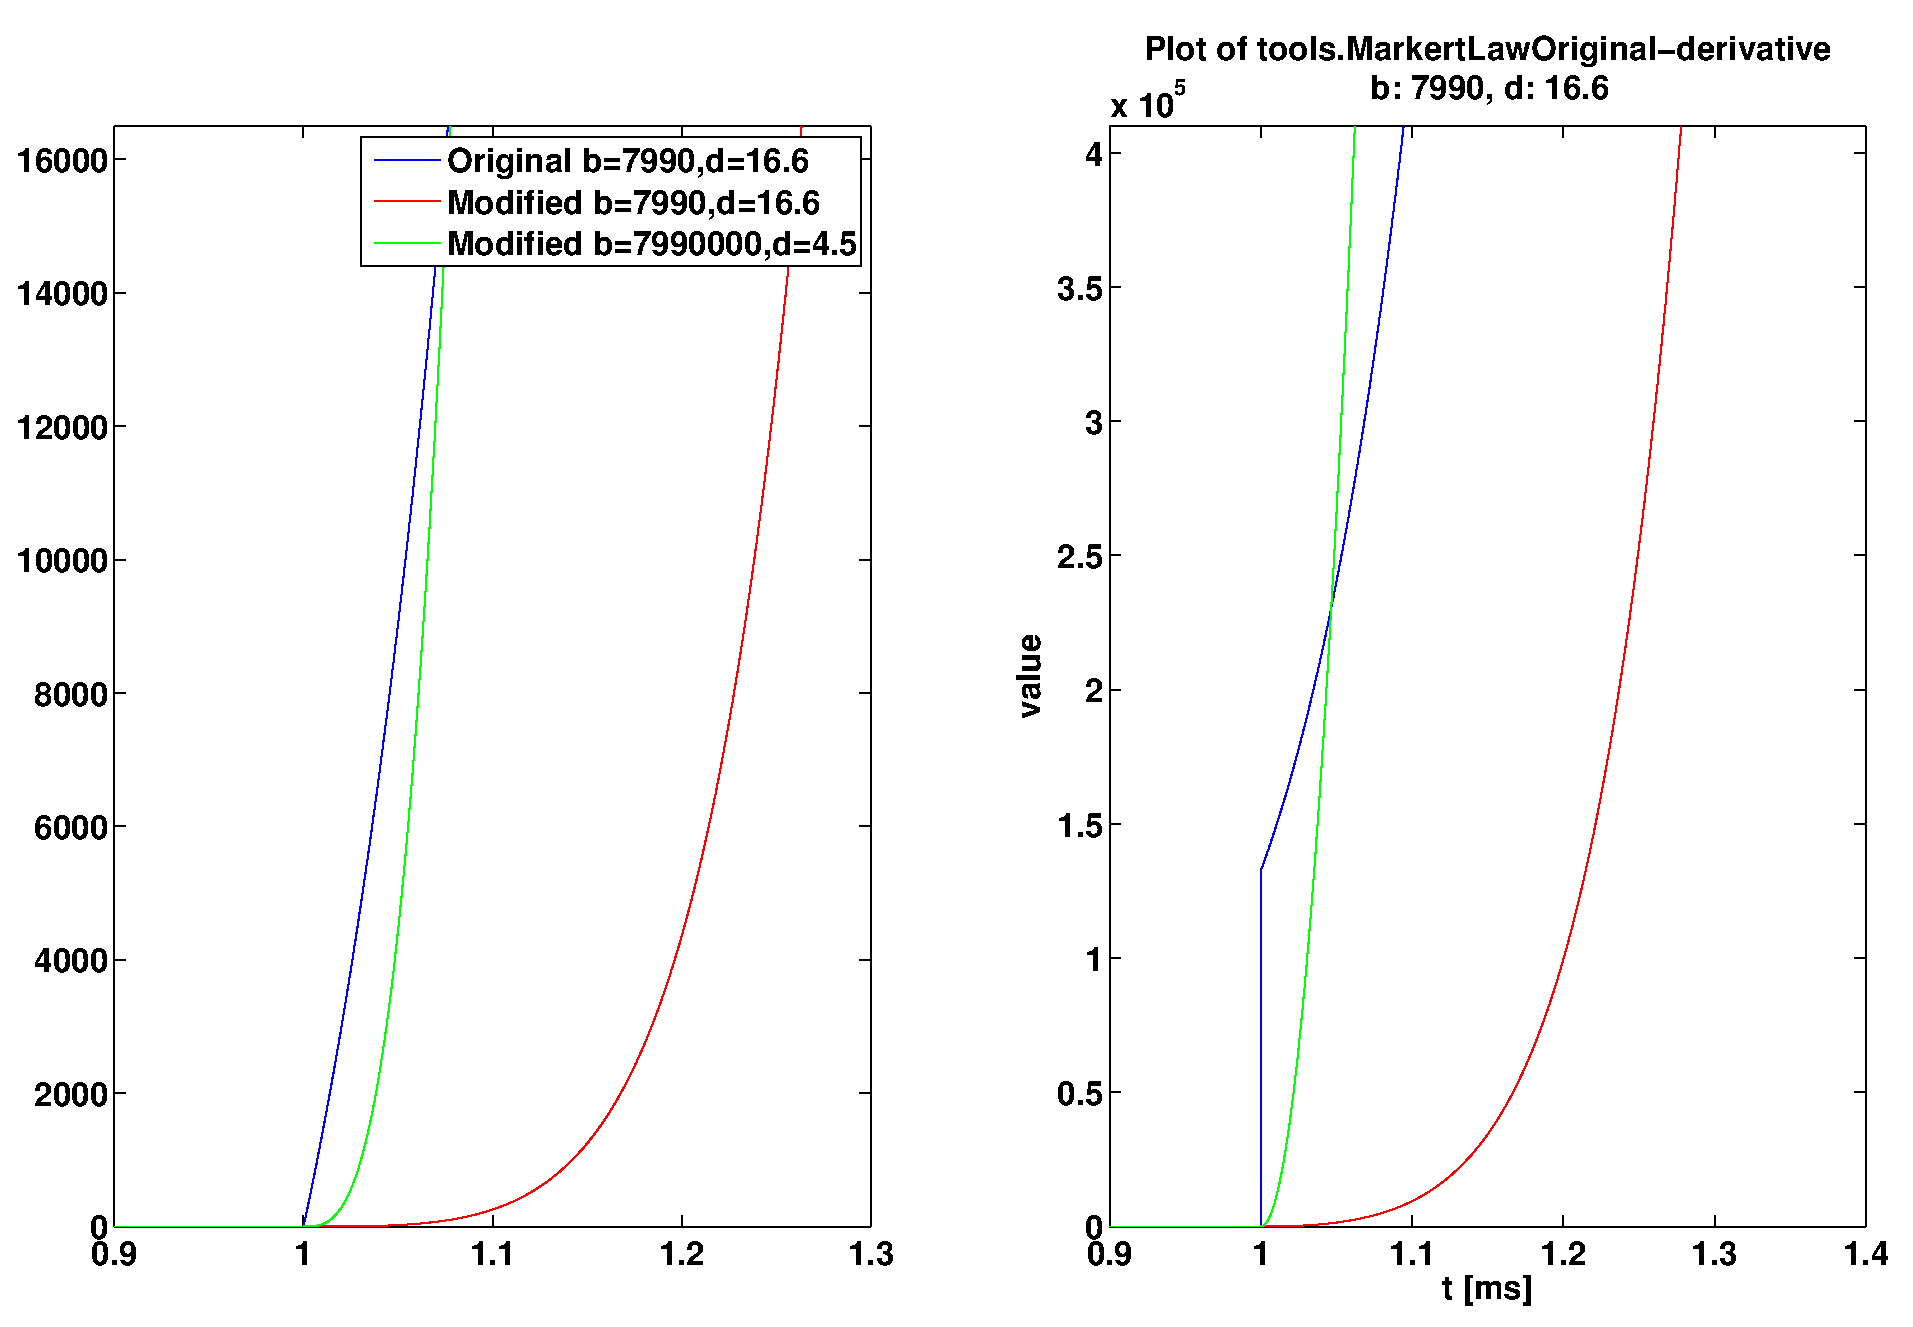
\includegraphics[width=\textwidth]{MarkertLawOriginal}
	\caption{Markert law for $b_1=7990 [kPa]$ and $d_1=16.6 [-]$. Discontinuous derivative at $\lambda=1$ with gap size $b_1d_1=132634 [kPa]$}
	\label{fig:steepmarkert}
\end{figure}

\subsubsection{Active force tensor $\vSf$}\label{sec:active_force}
We further assume to have a muscle activation $\alpha(X,t) \in [0,1]$, which is given by manual settings or motorunit models.
We then define
\begin{align}
	\Psi(\la) &:= \intl{0}{\la} p^{act}(s)ds,\nonumber\\
	p^{act}(\la) &:= p^{max}f_l(\la)f_v(\dla)\alpha(X,t),\nonumber\\
	f_l(\la) &:= \begin{cases}
		-\frac{25}{4}\left(\frac{\la}{\lfo}\right)^2 + \frac{25}{2}\frac{\la}{\lfo} - 5.25 & 0.6 \leq \frac{\la}{\lfo} \leq 1.4\\ 
		0 & \text{else}
	\end{cases} \label{def:fl},\\
	f_v(\dla) &:= ??,
\end{align}
with maximum pressure $p^{max} = 7.3 \left[\frac{N}{cm^2}\right] = 73~[kPa]$ and.
Similar to \eqref{eq:dpsidC} we obtain
\begin{align}
	\d{\Psi}{\vC}(\la) &= \frac{p^{max}}{2\la}f_l(\la)f_v(\dla)\alpha(X,t)\va_0\otimes\va_0
\end{align}
This gives
\begin{align}
	\vSf(X,t) &= \frac{p^{max}}{\la(X,t)}f_l(\la(X,t))f_v(\dla(X,t))\alpha(X,t)\va_0(X)\otimes\va_0(X)\\
	\vPf(X,t) &= \frac{p^{max}}{\la(X,t)}f_l(\la(X,t))f_v(\dla(X,t))\alpha(X,t)\vF(X,t)\va_0(X)\otimes\va_0(X)
\end{align}

\subsubsection{Viscous damping tensor $\vSv$/$\vPv$}
We introduce the viscous part of the stress tensor in the current configuration by defining
\begin{align}
\vPv(X,t) := \eta\,\dot{\vF}(X,t) \,,
\end{align}
where $\eta$ is a parameter describing the viscosity. 
\\
For the second Piola-Kirchhoff tensor that means
\begin{align}
\vSv(X,t) := \eta\,\vF^{-1}\dot{\vF}(X,t) \,.
\end{align}

\subsubsection{Overall stress tensor}
Adding the different parts together as given in \eqref{def:S_split} now gives
\begin{align}
	\vS(X,t) &= p(X,t)\vC^{-1}(X,t) + 2(c_{10} + I_1c_{01})\vI - 2c_{01}\vC(X,t)\label{def:overallS}\\
			 &\quad+\Biggl[\frac{b_1}{\la^2(X,t)}\left(\la^{d_1}(X,t) - 1\right)\nonumber\\
			 &\quad+\frac{p^{max}}{\la(X,t)}f_l(\la(X,t))f_v(\dla)\alpha(X,t)\Biggr]\va_0(X)\otimes\va_0(X)\\
			 &\quad+\vSv(X,t)\nonumber\\
	g(\la,\dla,\alpha)&:= \frac{b_1}{\la^2}\left(\la^{d_1} - 1\right)
		+\frac{p^{max}}{\la}f_l(\la)f_v(\dla)\alpha\label{def:g}\\			 
	\vP(X,t) &= \vF(X,t)\vS(X,t)\label{def:completeP}\\
			 &= p(X,t)\vF^{-T}(X,t) + 2(c_{10} + I_1(\vC(X,t))c_{01})\vF(X,t) - 2c_{01}\vF(X,t)\vC(X,t)\nonumber\\
			 &\quad+g(\la(X,t),\dla(X,t),\alpha(X,t))\vF(X,t)\va_0(X)\otimes\va_0(X)+\eta\,\dot{\vF}(X,t)\nonumber
\end{align}

\subsubsection{Initial conditions}
The reference configuration is \e{stress-free}, which means that $\vP(X,t) = \vS(X,t) = 0$.
With the incompressibility conditions we also have
\begin{align*}
	\vF(X,0) &= \vC(X,0) = \vI_3, & \det(\vF(X,0)) &= 1\\
	I_1(\vC(X,0)) &= \tr(\vI_3) = 3, & I_4(\vC(X,0),\va_0) & = \vI_3 : \va_0(X)\otimes\va_0(X)\\
		\dot{\vF(X,0)}&=\vnull,&&	= \tr(\va_0(X)\otimes\va_0(X)) = \no{\va_0}^2 = 1,\\
		\la(X,0) &= 1, f_l(1) = 1, f_v(1) = 1, & \alpha(X,0) &= 0,
\end{align*}
Hence we obtain from \eqref{def:overallS}
\begin{align}
	0 &= \vS(X,0) = p(X,0)\vI + 2(c_{10} + 3c_{01})\vI - 2c_{01}\vI\\
			 &\quad+\left(\frac{b_1}{1}\left(1 - 1\right)+\frac{p^{max}}{1}1\cdot1\cdot0\right)\va_0(X)\otimes\va_0(X)
			 +\eta\vI\vnull\nonumber\\
			 & = (p(X,0) + 2c_{10} + 4c_{01})\vI\\
			 p(X,0) &= -(2c_{10} + 4c_{01})
\end{align}

% \subsubsection{Detour}
% Prescribing $\vP$ will yield the behaviour of the overall system.
% The equation $\eqref{def:T}$ also holds for values in the current configuration, i.e.
% \[
% 	\vt(x,t,n) = \vsig(x,t)n,
% \]
% where $\vsig$ is the symmetric \e{Cauchy stress tensor}.


\section{FEM discretization}
\subsection{Domain decomposition, basis functions and master reference volume}
We specify a master hexahedron/volume/element $\Om = [-1,1]^3$ with corners
\begin{align*}
	\vX_{master} := \m{-1 & 1 & -1 & 1 & -1 & 1 & -1 &1\\-1 & -1 & 1 & 1 & -1 & -1 & 1 &1\\-1 & -1 & -1 & -1 & 1 & 1 & 1 &1\\}.
\end{align*}
This will be the ``natural'' order when referring to corners of the master volume, and we will stick with that order also for basis function indexing and all derived quantities.
All integrals will be performed on this master element $\Om$, where we apply a Gauss Quadrature with
\begin{align}
	X_1,\ldots,X_G  &\in \Om &&\text{Gauss points},\\
	w_1,\ldots,w_G  &\in \R &&\text{Gauss weights},
\end{align}
so that
\begin{align}
	\intom f(X)dX \approx \sumgp w_pf(X_p)\label{def:gaussintapprox}
\end{align}
for any integrable $f(X)$.
\subsubsection{Master basis functions}
\paragraph{Linear master basis functions}
For $\H^1$ we define the $n_b=8$ linear basis functions
\begin{align*}
	N_i:\Om &\to [0,1]\\
	N_i(X)  &= (1+(-1)^{i}X_1)(1+(-1)^{\ceil{\frac{i}{2}}}X_2)(1+(-1)^{\ceil{\frac{i}{4}}}X_3),\quad i=1\ldots n_b
\end{align*}
which amounts to trilinear functions equal to one in each corner of the hexahedron.
The set of functions has the property
\begin{align}
	\suml{i=1}{n_b}N_i &\equiv 1 & \text{i.e.}\quad \suml{i=1}{n_b}N_i(X) &= 1 \fo X\in\Om,\label{eq:basisfunsum}
\end{align}
which will be needed later.
\paragraph{Quadratic master basis functions}
For quadratic basis functions we need more Degrees of Freedom (DoF) in order to be able to satisfy \eqref{eq:basisfunsum}.
Well-known are $n_b=20$ or $n_b=27$ DoFs using extra edge-midpoint and mid-face locations.
We will use $n_b = 20$ with extra DoFs on the $12$ edge-midpoints.
Those be easily computed by a transformation matrix $T\in\R^{20 \times 8}$: 
\begin{lstlisting}
i = [1 2  2  3  4  4  5  5 6  7  7 8  9  9 10 10 11 11 12 12 13 14 14 15 16 16 17 17 18 19 19 20];  
j = [1 1  2  2  1  3  2  4 3  3  4 4  1  5 2  6  3  7  4  8  5  5  6  6  5  7  6  8  7  7  8  8];
s = [1 .5 .5 1 .5 .5 .5 .5 1 .5 .5 1 .5 .5 .5 .5 .5 .5 .5 .5 1  .5 .5 1  .5 .5 .5 .5 1  .5 .5 1];
T = sparse(i,j,s,20,8);
\end{lstlisting}
Then the extended ``corner'' set for the master hexahedron is $\vX_{master}T' \in\R^{20\times 3}$.
Now, for $\H^1$ we define the quadratic basis functions
\begin{align*}
	N_i:\Om &\to [0,1]\\
	N_1(X)  &= \frac{1}{8}(1-X_1)(1-X_2)(1-X_3)(-X_1-X_2-X_3-2)\\ % C1
    N_2(X)  &= \frac{1}{4}(1-X_1^2)(1-X_2)(1-X_3)\\ % E2
    N_3(X)  &= \frac{1}{8}(1+X_1)(1-X_2)(1-X_3)(X_1-X_2-X_3-2)\\ % C3
    N_4(X) &= \frac{1}{4}(1-X_2^2)(1-X_1)(1-X_3)\\ % E4
    N_5(X) &= \frac{1}{4}(1-X_2^2)(1+X_1)(1-X_3)\\ % E5
    N_6(X) &= \frac{1}{8}(1-X_1)(1+X_2)(1-X_3)(-X_1+X_2-X_3-2)\\ % C6
    N_7(X) &= \frac{1}{4}(1-X_1^2)(1+X_2)(1-X_3)\\ % E7
    N_8(X) &= \frac{1}{8}(1+X_1)(1+X_2)(1-X_3)(X_1+X_2-X_3-2)\\ % C8
    N_9(X) &= \frac{1}{4}(1-X_3^2)(1-X_1)(1-X_2)\\ % E9    
    N_{10}(X) &= \frac{1}{4}(1-X_3^2)(1+X_1)(1-X_2)\\ % E10
    N_{11}(X) &= \frac{1}{4}(1-X_3^2)(1-X_1)(1+X_2)\\ % E11
    N_{12}(X) &= \frac{1}{4}(1-X_3^2)(1+X_1)(1+X_2)\\ % E12
    N_{13}(X) &= \frac{1}{8}(1-X_1)(1-X_2)(1+X_3)(-X_1-X_2+X_3-2)\\ % C13
    N_{14}(X) &= \frac{1}{4}(1-X_1^2)(1-X_2)(1+X_3)\\ % E14
    N_{15}(X) &= \frac{1}{8}(1+X_1)(1-X_2)(1+X_3)(X_1-X_2+X_3-2)\\ %C15
    N_{16}(X) &= \frac{1}{4}(1-X_2^2)(1-X_1)(1+X_3)\\ % E16
    N_{17}(X) &= \frac{1}{4}(1-X_2^2)(1+X_1)(1+X_3)\\ % E17
    N_{18}(X) &= \frac{1}{8}(1-X_1)(1+X_2)(1+X_3)(-X_1+X_2+X_3-2)\\ % C18
    N_{19}(X) &= \frac{1}{4}(1-X_1^2)(1+X_2)(1+X_3)\\ % E19
    N_{20}(X) &= \frac{1}{4}(1+X_1)(1+X_2)(1+X_3)(X_1+X_2+X_3-2)]\\
\end{align*}
which amounts to triquadratic functions equal to one in each corner and edge-midpoints of the hexahedron.

\subsubsection{Domain decomposition}
Let $\Or$ be our domain of interest, decomposed into $\Or = \Omega_1\cup \ldots \cup \Omega_M$, where
$\Omega_m = [\vx^m_1,\ldots,\vx^m_{n_b}]$ is a deformed cube specified by the $n_b$ points $\vx_i^m\in\R^3$.
Let $\Ns := \{\vx_1,\ldots\vx_N\}$ denote the set of $N$ distinct nodes in
$\{\vx_1^1, \ldots, \vx_{n_b}^1, \vx_1^2, \ldots, \vx_{n_b}^{M-1}, \vx_1^M, \ldots, \vx_{n_b}^M\}$, numbered by first occurrence.

Using the notation
\begin{align}
	\vN(X) &:= \m{N_1(X) & \ldots & N_{n_b}(X)}^T\in\R^{n_b\times 1}\\
	\vX^m &:= \m{\vx^m_1 \ldots \vx^m_{n_b}} \in\R^{3\times n_b}
\end{align}
 we can specify an \e{isogeometric mapping} or diffeomorphism
\begin{align}
	\Phi_m : \Om &\to \Omega_m\\
	X &\mapsto \vX^m\vN(X)
\end{align}
which satisfies $\Omega_m = \Phi_m(\Or)$ and has the Jacobian
\begin{align}
	J\Phi_m(X) &= \m{\grad \Phi_{m_1}(X)\\\grad \Phi_{m_2}(X)\\\grad \Phi_{m_3}(X)\\} 
	= \vX^m\m{\grad N_1(X)\\ \vdots\\\grad N_{n_b}(X)} = \vX^m\nabla\vN(X) \in \R^{3\times 3}.\label{def:refbasis_jacobian}
\end{align}

\subsubsection{Node basis functions}
With the volume index set
\begin{align}
	%E_m &:= E(\Omega_m) := \{i\in\{1\ldots N\}~|~ \vx_i\in\Omega_m\}, \quad m=1\ldots M,\\
	V_k &:= \bigl\{i\in\{1\ldots M\}~|~ \vx_k\in\Omega_i\bigr\},&&k=1\ldots N
	%\Nk &:= \{i\in\{1\ldots N\}~|~ \vx_i\in E_m, m\in V_k\} = \{i ~|~ \supp\varphi_i \cap \supp\varphi_k \neq\es\},
\end{align}
we now define basis functions $\varphi_k$ on each node $k$ via
\begin{align}
	\varphi_k(X) &:= \begin{cases}
		N_{l(k,m)}(\Phi^{-1}_m(X)), & X\in\Omega_m, m\in V_k,\\
		0 & \text{else},	
	\end{cases}\label{def:referencebasisfun}\\
	l(k,m) &:= \{i\in\{1\ldots n_b\}~|~ N_i(\Phi_m^{-1}(\vx_k))=1\},\quad m=1\ldots M.
\end{align}
Here $l(k,m)$ refers to the local corner index of the basis function on $\Omega_m$ that equals one at $\vx_k$.


For the gradient of $\varphi_k$ we thus obtain
\begin{align}
	\grad\varphi_k(X) &\re{def:referencebasisfun} \grad (N_{l(k,m)}(\Phi^{-1}_m(X)))
					  = \grad N_{l(k,m)}(\Phi^{-1}_m(X))J\Phi^{-1}_m(X)\nonumber\\
					  &= \grad N_{l(k,m)}(\Phi^{-1}_m(X))(J\Phi_m(X))^{-1}\label{eq:gradvarphi}
\end{align}
for $X\in\Omega_m, m\in V_k$ (zero otherwise).
 
\subsubsection{Discrete integrals with node basis functions}
We define the shorthands
\begin{align}
	\pmp &:= \Phi_m(X_p)\\
	\jmp &:= |\det J\Phi_m(X_p)| = |\det \vX^m\nabla\vN(X_p)|.\label{def:jacshorthand}\\
	\dNkmp &:= \nabla\varphi_k(\pmp) \re{eq:gradvarphi} \left(J\Phi_m(X_p)\right)^{-T}\nabla \Nkmp)\in\R^3\label{}
\end{align}

With the above, and the transformation theorem and the local support of the basis function $\varphi_k$ we now have for any integrable $f(X,t)$ that
\begin{align}
   \intl{\Or}{}f(X,t)\varphi_k(X)dX &= \suml{m=1}{M}\intl{\Omega_m}{}f(X,t)\varphi_k(X)dX = \sumvk\intl{\Omega_m}{}f(X,t)\varphi_k(X)dX\nonumber\\
    &= \sumvk\intl{\Phi_m(\Omega)}{}f(X,t)\varphi_k(X)dX\nonumber\\
	&= \sumvk\intl{\Om}{}f(\Phi_m(X),t)\varphi_k(\Phi_m(X))|\det J\Phi_m(X)|dX\nonumber\\
	& \re{def:gaussintapprox} \sumvk\sumgp w_pf(\pmp,t)\varphi_k(\pmp)|\det J\Phi_m(X_p)|\nonumber\\
	& \re{def:referencebasisfun} \sumvk\sumgp w_pf(\pmp,t)N_{l(k,m)}(\Phi_m^{-1}(\pmp))|\det J\Phi_m(X_p)|\nonumber\\
	& \re{def:jacshorthand} \sumvk\sumgp w_pf(\pmp,t)\Nkmp\jmp\label{eq:fphidx}
\end{align}

Similarly we obtain for the gradient that
\begin{align}
	\intl{\Or}{}f(X,t)\nabla\varphi_k(X)dX &= \sumvk\sumgp w_pf(\pmp,t)\dNkmp\jmp\label{eq:fgradphidx}
\end{align}

\subsection{Weak form and linear ansatz}
For discretization we use taylor-hood elements, which means $C^2(\Or)$ test/ansatz functions for the displacement and $C^1(\Or)$ test/ansatz functions for
the pressure.
We fix nodes $\{\vx_1,\ldots,\vx_N\}$, the test space $\H^2$ spanned by $C^2(\Or)$ test functions
$\varphi_1,\ldots,\varphi_N$ and the test space $\H^1$ spanned by $C^1(\Or)$ test functions
$\psi_1,\ldots,\psi_N$. 
We have $\varphi_i(\vx_j) = \delta_{ij}$ and $\varphi_k \equiv 0$ on $\partial\Or$ for all $k$, which holds true for $\psi_i$ as well.
Now, equation \eqref{def:maineq} (without body forces) and the incompressibility constraint give the system 
\begin{align}
	\rho_0(X)\d{\vV}{t}(X,t) &= \divergence\vP(X,t) \qquad \fo X\in\Or,\\
	J(X,t) &= 1 \qquad \fo X\in\Or,
\end{align}
for which we have the spatial weak form
\begin{align}
	\intor\rho_0(X)\d{\vV}{t}(X,t)\varphi(X)dX &= \intor\divergence\vP(X,t)\varphi(X)dX &&\fo \varphi\in\H^2\\
	\intor (J(X,t)-1)\psi(X)dX &= 0 && \fo \psi\in\H^1
\end{align}
The right hand side can be transformed as
\begin{align*}
	\intor \div{\vP(X,t)}\varphi(X) dX &= \intor \div{\vP(X,t)\varphi(X)} - \vP(X,t)\divergence\varphi(X) dX\\
		 &= \underbrace{\intorb \vP(X,t)\varphi(X) dN}_{=0} - \intor \vP(X,t)\divergence\varphi(X)dX\\
		 &= \intor -\vP(X,t)\divergence\varphi(X) dX
\end{align*}
As $\H$ is spanned by linear independent $\varphi_k$,
this gives $3N+N$ equations (for each test function $\varphi_k$, 3D displacement and one constraint) as
\begin{align}
	\intor \rho_0(X)\d{\vV}{t}(X,t)\varphi_k(X)dX + \intor\vP(X,t)\dpk dX &= \vnull && \fo k=1\ldots N\label{def:weakform}\\
	\intor (J(X,t)-1)\psi_k(X)dX &= 0 && \fo k=1\ldots N\label{def:weakform_nb}
\end{align}

Now as solution space we choose the linear ansatz $\chi\in\H^2, p\in\H^1$ as
\begin{align}
	\chi(X,t) &= \sumi \vc_i(t)\varphi_i(X), && \vc_i(t):[0,T] \to\R^3.\\
	p(X,t) &= \sumi d_i(t)\psi_i(X), && d_i(t):[0,T] \to\R.
\end{align}
With this we have
\begin{align}
	\vV(X,t) &= \d{\chi}{t}(X,t) = \sumi \vc_i'(t)\varphi_i(X)\\
	\vA(X,t) &= \d{\vV}{t}(X,t) = \sumi \vc_i''(t)\varphi_i(X)\\
	\vF(X,t) &= \d{\chi}{X}(X,t) = \m{\grad \chi_1(X,t)\\ \grad \chi_2(X,t)\\ \grad \chi_3(X,t)}
		   = \sumi\m{c_{i,1}\d{\varphi_i}{X_1} & \dots & c_{i,1}\d{\varphi_i}{X_3}\\
		   				\vdots & \ddots & \vdots\\
		   				c_{i,3}\d{\varphi_i}{X_1} & \dots & c_{i,3}\d{\varphi_i}{X_3}}\\
		   &=\sumi \vc_i(t)\cdot \grad\varphi_i(X) = \sumi \vc_i(t)\otimes \dpi.
\end{align}
This can be used to derive the quantities
\begin{align}
	I_1(\vC(X,t)) &= \tr\vC(X,t) = \tr(\vF(X,t)^T\vF(X,t)) = \vF(X,t) : \vF(X,t)\nonumber\\
	&= \sumi \vc_i(t)\otimes \dpi : \sumi \vc_i(t)\otimes \dpi\nonumber\\
	&= \sumi\sumj \left(\vc_i(t)\otimes \dpi\right) : (\vc_j(t)\otimes \dpj)\nonumber\\
	&= \sumi\sumj (\vc_i(t) \cdot \vc_j(t))(\dpi \cdot \dpj)\label{eq:I1_basis}\\
	\vF(X,t)^T\vF(X,t) &= \sumi\sumj \bigl(\vc_i(t)\otimes\dpi\bigr)^T\vc_j(t)\otimes\dpj\nonumber\\
	 &= \sumi\sumj \bigl(\dpi\otimes\vc_i(t)\bigr)\vc_j(t)\otimes\dpj\nonumber\\
	 &=\sumi\sumj (\vc_i(t)\cdot \vc_j(t))\dpi\otimes\dpj\nonumber\\
	\lambda_f(X,t)^2 &=I_4(\vC(X,t),a_0(X)) = \vC(X,t):(a_0(X)\otimes a_0(X))\nonumber\\
			&=  \vF(X,t)^T\vF(X,t) : (a_0(X)\otimes a_0(X))\nonumber\\
			&=  \sumi\sumj (\vc_i(t)\cdot \vc_j(t))\bigl(\dpi\otimes\dpj\bigr) : (a_0(X)\otimes a_0(X))\nonumber\\
			&=  \sumi\sumj (\vc_i(t)\cdot \vc_j(t))\left(\dpi\cdot a_0(X)\right)(\dpj\cdot a_0(X))\label{eq:lambdaf_basis}\\
	\d{\lambda_f^2}{t}(X,t) &= 2\lambda_f \suml{i,j}{N} (\vc'_i(t)\cdot \vc_j(t) + \vc_i(t)\cdot \vc'_j(t))\left(\dpi\cdot a_0(X)\right)(\dpj\cdot a_0(X))\nonumber\\
		&= 4\lambda_f \suml{i,j}{N} (\vc_i(t)\cdot \vc'_j(t))\left(\dpi\cdot a_0(X)\right)(\dpj\cdot a_0(X))\nonumber\\
    \vF(X,t)\vF(X,t)^T\vF(X,t) &= \sumk\vc_k(t)\otimes\dpk\sumi\sumj (\vc_i(t)\cdot \vc_j(t))\dpi\otimes\dpj\nonumber\\
    	&= \suml{i,j,k}{N}(\vc_i(t)\cdot \vc_j(t))(\vc_k(t)\otimes\dpk)\dpi\otimes\dpj\nonumber\\
    	&= \suml{i,j,k}{N}(\vc_i(t)\cdot \vc_j(t))(\dpk\cdot\dpi)(\vc_k(t)\otimes\dpj)\nonumber\\
    \vF(X,t)(\va_0(X)\otimes\va_0(X)) &= \sumi \vc_i(t)\otimes \dpi(\va_0(X)\otimes\va_0(X))\nonumber\\
    &= \sumi (\vc_i(t)\otimes \va_0(X))(\dpi\cdot\va_0(X))\nonumber
\end{align}

\subsection{Domain decomposition, basis functions and master reference volume}
We specify a master reference volume $\Om = [-1,1]^3$, and for $\H^1$ the basis functions
\begin{align*}
	N_i:\Om &\to [0,1]\\
	N_i(X)  &= (1+(-1)^{i}X_1)(1+(-1)^{\ceil{\frac{i}{2}}}X_2)(1+(-1)^{\ceil{\frac{i}{4}}}X_3),\quad i=1\ldots 8
\end{align*}
which amounts to trilinear functions equal to one in each corner of the hexahedron having the property
\begin{align}
	\suml{i=1}{8}N_i &\equiv 1 & \text{i.e.}\quad \suml{i=1}{8}N_i(X) &= 1 \fo X\in\Om.
\end{align}

We further specify a decomposition $\Or = \Omega_1\cup \ldots \cup \Omega_M$, where
$\Omega_m = [\vx^m_1,\ldots,\vx^m_8]$ is a deformed cube specified by the eight corner points $\vx_i^m\in\R^3$.
Using the notation
\begin{align}
	\vN(X) &:= \m{N_1(X) & \ldots & N_8(X)}^T\in\R^{8\times 1}\\
	\vX^m &:= \m{\vx^m_1 \ldots \vx^m_8} \in\R^{3\times 8}
\end{align}
 we can specify an \e{isogeometric mapping} or diffeomorphism
\begin{align}
	\Phi_m : \Om &\to \Omega_m\\
	X &\mapsto \vX^m\vN(X)
\end{align}
which satisfies $\Omega_m = \Phi_m(\Or)$ and has the Jacobian
\begin{align}
	J\Phi_m(X) &= \m{\grad \Phi_{m_1}(X)\\\grad \Phi_{m_2}(X)\\\grad \Phi_{m_3}(X)\\} 
	= \vX^m\m{\grad N_1(X)\\ \vdots\\\grad N_8(X)} = \vX^m\nabla\vN(X) \in \R^{3\times 3}.\label{def:refbasis_jacobian}
\end{align}
 
With the edge/volume/neighbor index sets
\begin{align}
	E_m &:= E(\Omega_m) := \{i\in\{1\ldots N\}~|~ \vx_i\in\Omega_m\}, \quad m=1\ldots M,\\
	V_k &:= V(\vx_k) := \{i\in\{1\ldots M\}~|~ \vx_k\in\Omega_i\}, \quad k=1\ldots N,\\
	\Nk &:= \{i\in\{1\ldots N\}~|~ \vx_i\in E_m, m\in V_k\} = \{i ~|~ \supp\varphi_i \cap \supp\varphi_k \neq\es\},
\end{align}
we now define the basis functions $\varphi_k$ via
\begin{align}
	\varphi_k(X) &:= \begin{cases}
		N_{l(k,m)}(\Phi^{-1}_m(X)), & X\in\Omega_m, m\in V_k,\\
		0 & \text{else},	
	\end{cases}\label{def:referencebasisfun}\\
	l(k,m) &:= \{i\in\{1\ldots 8\}~|~ N_i(\Phi_m^{-1}(\vx_k))=1\},\quad m=1\ldots M.
\end{align}
Here $l(k,m)$ refers to the local corner index of the basis function on $\Omega_m$ that equals one at $\vx_k$.
For the gradient of $\varphi_k$ we thus obtain
\begin{align*}
	\nabla\varphi_k(X)^T &= \grad\varphi_k(X) \re{def:referencebasisfun} \grad (N_{l(k,m)}(\Phi^{-1}_m(X)))\\
					  &= \grad N_{l(k,m)}(\Phi^{-1}_m(X))J\Phi^{-1}_m(X) && X\in\Omega_m, m\in V_k
\end{align*}

We further apply a Gauss Quadrature on $\Om$ with
\begin{align}
	X_1,\ldots,X_G  &\in \Om &&\text{Gauss points},\\
	w_1,\ldots,w_G  &\in \R &&\text{Gauss weights},
\end{align}
so that
\begin{align}
	\intom f(X,t)dX \approx \sumgp w_pf(X_p).\label{def:gaussintapprox}
\end{align}
With the above and the transformation theorem we now have for any integrable $f(X,t)$ and the shorthand $\pmp := \Phi_m(X_p)$ that
\begin{align}
	\intl{\Omega_m}{}f(X,t)\varphi_k(X)dX &= \intl{\Phi_m(\Omega)}{}f(X,t)\varphi_k(X)dX\label{eq:fphidx}\\
	& = \intl{\Om}{}f(\Phi_m(X),t)\varphi_k(\Phi_m(X))|\det \nabla\Phi(X)|dX\nonumber\\
	& \re{def:gaussintapprox} \sumgp w_pf(\pmp,t)\varphi_k(\pmp)|\det \nabla\Phi(X_p)|\nonumber\\
	& \re{def:referencebasisfun} \sumgp w_pf(\pmp,t)N_{l(k,m)}(\Phi_m^{-1}(\pmp))|\det \nabla\Phi(X_p)|\nonumber\\
	& \re{def:refbasis_jacobian} \sumgp w_pf(\pmp,t)N_{l(k,m)}(X_p)|\det \vX^m\nabla\vN(X_p)|\nonumber
\end{align}
We further have
\begin{align}
	\nabla\varphi_k(\pmp)^T &= \grad N_{l(k,m)}(\Phi^{-1}_m(\pmp))J\Phi^{-1}_m(\pmp)\nonumber\\
		&= \grad N_{l(k,m)}(X_p))J\Phi^{-1}_m(\Phi_m(X_p))\nonumber\\
		&= \grad N_{l(k,m)}(X_p))\left(J\Phi_m(X_p)\right)^{-1}\nonumber\\
	\nabla\varphi_k(\pmp) &= \left(J\Phi_m(X_p)\right)^{-T}\nabla N_{l(k,m)}(X_p))\nonumber\\
		&= (\vX^m\nabla\vN(X_p))^{-T}\nabla N_{l(k,m)}(X_p)\\
		&=: \dNkmp \in\R^3\\
	\intl{\Omega_m}{}f(X,t)\nabla\varphi_k(X)dX &= \sumgp w_pf(\pmp,t)\dNkmp|\det \vX^m\nabla\vN(X_p)|\label{eq:fgradphidx}
\end{align}

\subsection{Application to weak form}
We introduce the shorthand
\begin{align}
	\jmp &:= |\det \vX^m\nabla\vN(X_p)|.\label{def:jacshorthand}
\end{align}
Finally, for a fixed $k\in\{1,\ldots, N\}$ we have for the first term of \eqref{def:weakform}:
\begin{align*}
	\intor \rho_0(X)\d{\vV}{t}(X,t)\varphi_k(X)dX
		&= \suml{m=1}{M}\intl{\Omega_m}{} \rho_0(X)\d{\vV}{t}(X,t)\varphi_k(X)dX\\
		&= \sumvk\intl{\Omega_m}{} \rho_0(X)\d{\vV}{t}(X,t)\varphi_k(X)dX\\  		
		&= \sumvk\intl{\Omega_m}{} \rho_0(X)\sumi \vc_i''(t)\varphi_i(X)\varphi_k(X)dX\\
		&\re{eq:fphidx} \sumvk\sumgp w_p \rho_0(\pmp)\sumi \vc_i''(t)\varphi_i(\pmp) N_{l(k,m)}(X_p)\jmp\\
		&= \sumvk\sumnk \vc_i''(t)\sumgp w_p \rho_0(\pmp)N_{l(i,m)}(X_p) N_{l(k,m)}(X_p)\jmp
\end{align*}

The second term of \eqref{def:weakform}, with \eqref{def:completeP}, reads as
\begin{align*}
		&\intor\vP(X,t)\dpk dX\\
		=& \suml{m=1}{M}\intl{\Omega_m}{}\vP(X,t)\dpk dX
			= \sumvk\intl{\Omega_m}{}\vP(X,t)\dpk dX\\
		\re{eq:fgradphidx}&\sumvk\sumgp w_p\vP(\pmp,t)\dNkmp|\det \vX^m\nabla\vN(X_p)|\\
		\re{def:jacshorthand}&\sumvk\sumgp w_p\vP(\pmp,t)\dNkmp\jmp\\
		\re{def:completeP}&\sumvk\sumgp w_p\Bigl[p(\pmp,t)\vF^{-T}(\pmp,t) + 2(c_{10} + I_1(\vC(\pmp,t))c_{01})\vF(\pmp,t)\\
			 &- 2c_{01}\vF(\pmp,t)\vC(\pmp,t)+g(\lambda_f(\pmp,t))\vF(\pmp,t)\va_0(\pmp)\otimes\va_0(\pmp)\Bigr]\dNkmp\jmp\nonumber.
\end{align*}
In detail we have
\begin{align*}
	I_1(\vC(\pmp,t)) &\re{eq:I1_basis} \sumi\sumj (\vc_i(t) \cdot \vc_j(t))(\divergence\varphi_i(\pmp) \cdot \divergence\varphi_j(\pmp))\\
	&\re{def:referencebasisfun} \suml{i,j\in E_m}{} (\vc_i(t) \cdot \vc_j(t))(\divergence\varphi_i(\pmp) \cdot \divergence\varphi_j(\pmp))\\
	%&\re{def:referencebasisfun} \suml{i,j\in E_m}{} (\vc_i(t) \cdot \vc_j(t))(\nabla N_{l(i,m)}(X_p) \cdot \nabla N_{l(j,m)}(X_p))\\
	\vF(\pmp,t)\vC(\pmp,t) &= \vF(\pmp,t)\vF(\pmp,t)^T\vF(\pmp,t)\\
    	&= \suml{i,j,k}{N}(\vc_i(t)\cdot \vc_j(t))(\divergence\varphi_k(\pmp)\cdot\divergence\varphi_i(\pmp))(\vc_k(t)\otimes\divergence\varphi_j(\pmp))\\
    	%&= \suml{i,j,q\in E_m}{}(\vc_i(t)\cdot \vc_j(t))(\nabla N_{l(q,m)}(X_p)\cdot\nabla N_{l(i,m)}(X_p))(\vc_q(t)\otimes\nabla N_{l(j,m)}(X_p))\\
    \lambda_f(\pmp,t)^2 &\re{eq:lambdaf_basis}
    		\sumi\sumj (\vc_i(t)\cdot \vc_j(t))\left(\divergence\varphi_i(\pmp)\cdot a_0(\pmp)\right)(\divergence\varphi_j(\pmp)\cdot a_0(\pmp))\nonumber\\
    	%&= \suml{i,j\in E_m}{} (\vc_i(t)\cdot \vc_j(t))\left(\nabla N_{l(i,m)}(X_p)\cdot a_0(\pmp)\right)(\nabla N_{l(j,m)}(X_p))\cdot a_0(\pmp))\nonumber
%\end{align*} 
%\begin{align*}  	
    \vF(\pmp,t)(\va_0(\pmp)\otimes\va_0(\pmp)) 
    	&= \sumi (\vc_i(t)\otimes \va_0(\pmp))(\divergence\varphi_i(\pmp)\cdot\va_0(\pmp))\nonumber\\
    	%&= \suml{i\in E_m}{} (\vc_i(t)\otimes \va_0(\pmp))(\nabla N_{l(i,m)}(X_p)\cdot\va_0(\pmp))\nonumber
\end{align*}
By the same arguments, condition/equation \eqref{def:weakform_nb} now reads as
\begin{align*}
	\intor (J(X,t)-1)\psi_k(X)dX &= \sumvk\sumgp w_p (\det\vF(\pmp,t)-1) N_{l(k,m)}(X_p)\jmp\\
	&= \sumvk\sumgp w_p \left(\det\left(\sumi \vc_i(t)\otimes \divergence\varphi_i(\pmp)\right)-1\right) N_{l(k,m)}(X_p)\jmp\\
	&= \sumvk\sumgp w_p \left(\det\left(\sum_{i\in E_m} \vc_i(t)\otimes \divergence\varphi_i(\pmp)\right)-1\right) N_{l(k,m)}(X_p)\jmp.\\
\end{align*}


\section{Formulation as System of ODEs}\label{sec:odeform}
We now collect the $N$ position coefficient vectors $\vc_i \in\R^3$ and pressure coefficients as
\begin{align*}
	\vu(t) &:= (\vc_1^T(t) \ldots \vc_N^T(t))^T \in\R^{3N},\\
	\vw(t) &:= (d_1(t) \ldots d_{N_P}(t))^T \in\R^{N_P}.
\end{align*}
We introduce the triple index
\begin{align}
	[i] &:= 3(i-1)+(1~2~3)^T, \text{ i.e.}\\
	\vu[i] &:= (\vu_{3(i-1)+1}~~\vu_{3(i-1)+2}~~\vu_{3(i-1)+3})^T\in\R^{3\times 1}
\end{align}
for the $x,y,z$ components of the $i$-th coefficient and hence identify
\[
	\vF(X,t) = \sumi \vc_i(t)\otimes \nabla\varphi_i(X) = \sumi \vu[i](t)\otimes \nabla\varphi_i(X) =: \vF(X,\vu(t)).
\]

From \eqref{def:discreteVphidX} we obtain a mass matrix $\vM\in\R^{3N\times 3N}$ via the operator $\vM$:
\begin{align*}
  \vM[k](\vu(t)) &:= \sumi \vc_i''(t)\sumvk\sumgp w_p \rho_0(\pmp)N_{l(i,m)}(X_p) \Nkmp\jmp, && k=1\ldots N,\\
	\vM\bigl[[i],[k]\bigr] &:= \m{1&0&0\\0&1&0\\0&0&1} \sumvk\sumgp w_p \rho_0(\pmp)N_{l(i,m)}(X_p) \Nkmp\jmp, && i,k=1\ldots N.
\end{align*}
	
We now split the stress tensor into a nonlinear and a linear part:
\begin{align}
  \vP(X,t) &= \underbrace{p(X,t)\vF^{-T}(X,t) + \vPi + \vPa + \vPf}_{\displaystyle=:\vPnl} + \underbrace{\vPv}_{\displaystyle=:\vPl}
  \label{def:splitPnllin}
\end{align}
For the linear part, we obtain with \eqref{def:discretePgradphidX} the damping matrix $\vD\in\R^{3N\times 3N}$ via the operator $\vD$:
\begin{align}
    \vD[k](\vu(t))&:=
		\intor\vPl(X,t)\dpk dX \nonumber\\
		&=\sumvk\sumgp w_p\vPl(\pmp,t)\dNkmp\jmp\nonumber\\
		&=\sumvk\sumgp w_p \eta \sumi \vc_i'(t) \otimes \dNimp \dNkmp\jmp\nonumber\\
		&=\sumi \vc_i'(t) \sumvk\sumgp w_p \eta \dNimp \cdot \dNkmp\jmp
		&& k=1\ldots N.\label{def:discretePviscgradphidX}
\end{align}
\begin{align*}
	\vD\bigl[[i],[k]\bigr] &:= \eta\m{1&0&0\\0&1&0\\0&0&1} \sumvk\sumgp w_p \dNimp \cdot \dNkmp \jmp, && i,k=1\ldots N.
\end{align*}

Also carrying the arguments through to $\vPnl(X,t) = \vPnl(X,\vu(t),\vw(t))$.
This allows us to define operators $\vK: \R^{3N\times N_P}\to\R^{3N}, \vg:\R^{3N}\to\R^{N_P}$ (by components) as
\begin{align}
	\vK[k](\vu(t),\vw(t)) &:= \intor\vPnl(X,\vu(t),\vw(t))\dpk dX\\
	&\re{def:discretePgradphidX} \sumvk\sumgp w_p\vPnl(\pmp,\vu(t),\vw(t))\dNkmp\jmp\in\R^3, && k=1\ldots N,\\
	\vg_k(\vu(t)) &:= \intor (\det\vF(X,\vu(t))-1)\psi_k(X)dX\\
	&\re{eq:weak_incomp_condition}\sumvk\sumgp w_p (\det\vF(\pmp,\vu(t))-1) \Nkmp\jmp, && k=1\ldots N_P.
\end{align}

Altogether, the system of equations \eqref{def:mainsys1_weak_kparts},\eqref{def:maineq_cond_weak_kparts} yields the constrained second order differential equation
or differential-algebraic equation (DAE)
\begin{align}
	\vM\vu''(t) + \vK(\vu(t),\vw(t)) + \vD\vu'(t) &= \vnull,\\
		\text{s.t.}\quad \vg(\vu(t)) &= \vnull,
\end{align}
which can be transformed to a first-order system with the substitution $\vv(t) := \vu'(t)$:
\begin{align}
	\m{\vI & \vnull\\ \vnull & \vM}\m{\vu'(t)\\ \vv'(t)} 
	&= \m{\vv(t) \\ -\vK(\vu(t),\vw(t))} - \m{\vnull &\vnull\\ \vnull &\vD \\}\m{\vu \\ \vv},\\
	\text{s.t.}\quad \vg(\vu(t))		&= \vnull.
\end{align}

\subsection{Time-discretization}
For the time-discretization we use the notation $\vu_i := \vu(t_i), t_i := i\Delta t, i=0\ldots N_t\in\N, \Delta t > 0$, similarly for $\vv,\vw$.
Using the standard backward-Euler scheme results in the implicit system
\begin{align}
	\frac{1}{\Delta t}\m{\vI & \vnull\\ \vnull & \vM}\m{\vu_{i+1}-\vu_i\\\vv_{i+1}-\vv_i} 
	&= \m{\vv_{i+1}\\-\vK(\vu_{i+1},\vw_{i+1})} - \m{\vnull &\vnull\\ \vnull &\vD \\}\m{\vu_{i+1} \\ \vv_{i+1}},\\
	\vg(\vu_{i+1})		&= \vnull.
\end{align}
Writing the overall system as 
\begin{align}
	\vf([\vu; \vv; \vw]) &:= \m{\frac{1}{\Delta t}\m{\vI & \vnull\\ \vnull & \vM}\m{\vu-\vu_i\\\vv-\vv_i} 
	+ \m{-\vv\\\vK(\vu,\vw)} + \m{\vnull &\vnull\\ \vnull &\vD \\}\m{\vu \\ \vv}\\
		\vg(\vu)},
\end{align}
we apply the standard Newton-Iteration
\begin{align}
	[\vu; \vv; \vw]^1 &:= [\vu_i; \vv_i; \vw_i],\\
	[\vu; \vv; \vw]^{n+1} &:= [\vu; \vv; \vw]^{n} - \nabla \vf([\vu; \vv; \vw]^n)^{-1}\vf([\vu; \vv; \vw]^n), 
\end{align}
to find $\vu_{i+1}$ etc.
Here we have the Jacobian
\begin{align}
	 \nabla \vf([\vu; \vv; \vw]) &:= \m{\frac{1}{\Delta t} \vI & -\vI & \vnull & \Bigl\rbrace3N\\
	 									\nabla_{\vu}\vK(\vu,\vw) & \frac{1}{\Delta t}\vM+\vD & \nabla_{\vw}\vK(\vu,\vw) & \Bigl\rbrace3N\\
	 									\underbrace{\nabla_{\vu}\vg(\vu)}_{3N} & \underbrace{\vnull}_{3N} & \underbrace{\vnull}_{N_P} & \Bigl\rbrace N_P}.
\end{align}

\subsection{Derivation of nonlinearity Jacobian}
Here are some important formulas for matrix derivatives. We first define
\begin{align}
    \vU^j_i(X) & := \m{\ve_i\otimes\dpj}, i=1\ldots3, &
	\vU^j_1(X) &= \m{
            ~   & \dpj  & ~ \\
            0   & 0                 & 0 \\
            0   & 0                 & 0
          },\\
  \vU^j_2(X) &= \m{
            0   & 0                 & 0 \\
            ~   & \dpj  & ~ \\            
            0   & 0                 & 0
          },& 
  \vU^j_3(X) & = \m{
            0   & 0                 & 0 \\
            0   & 0                 & 0 \\
            ~   & \dpj  & ~            
          }.
\end{align}
\begin{align}
	\vF(X,\vu + h\ve[j]_i) &= \vF(X,\vu) + \m{\vnull \\ h\dpj^T\\ \vnull}\leftarrow i\nonumber\\
	&= \vF(X,\vu) + h\ve_i\otimes\dpj\\
	&= \vF(X,\vu) + h\vU^j_i(X),\qquad i=1\ldots3,\ve_i\in\R^3 \text{ unit vec}\nonumber\\
	\Rightarrow \d{}{u[j]_i}\vF(X,\vu) &= \vU^j_i(X),\qquad i=1\ldots3\nonumber\\
	(\vS+\Delta\vU)^{-1} &= \vS^{-1} - \vS^{-1}\Delta\vU\vS^{-1} + \O{|\Delta U|^2}\qquad\cite[p.57]{Bonet2008}\label{eq:matrixinversederivative}\\
	\vF(X,\vu + h\ve[j]_i)^{-1} &= \left(\vF(X,\vu) + h\vU^j_i(X)\right)^{-1}\nonumber\\
		&\re{eq:matrixinversederivative}\vF(X,\vu)^{-1} - h\vF(X,\vu)^{-1}\vU^j_i(X)\vF(X,\vu)^{-1} + \O{h^2}\nonumber\\
	\Rightarrow\d{}{u[j]_i}\vF^{-1}(X,\vu) &= -\vF(X,\vu)^{-1}\vU^j_i(X)\vF(X,\vu)^{-1}\nonumber\\
	\Rightarrow\d{}{u[j]_i}\vF^{-T}(X,\vu) &= -\vF(X,\vu)^{-T}(\vU^j_i(X))^{T}\vF(X,\vu)^{-T}\nonumber
\end{align}

In detail, we have
% \begin{align*}
% 	\d{\vF}{\vu[k]}(X,\vu) &= \nabla_{\vu[k]}\vF(X,\vu)\\
% 			&= \nabla_{\vu[k]}\sumi \vu[i] \otimes \dpi = \bullet\otimes\dpk\\
% 	\nabla_{\vu[k]}(\det\vF(X,\vu)-1) &= \det(\vF(X,\vu))\vF(X,\vu)^{-1}:\nabla_{\vu[k]}\vF(X,\vu)\\
% 				&= \det(\vF(X,\vu))\vF(X,\vu)^{-1}:\bullet\otimes\dpk
% \end{align*}
\subsubsection{Derivation of $\nabla_{\vu}\vK(\vu,\vw)$}
\begin{align*}
	\nabla_{\vu}\vK(\vu,\vw) &= \m{\nabla_{\vu}\vK[1](\vu,\vw)\\ \vdots \\ \nabla_{\vu}\vK[N](\vu,\vw)}
	 = \m{\nabla_{\vu[1]}\vK[1](\vu,\vw) & \ldots & \nabla_{\vu[N]}\vK[1](\vu,\vw)\\
	 	\vdots & \ddots & \vdots\\
	   \nabla_{\vu[1]}\vK[N](\vu,\vw) & \ldots & \nabla_{\vu[N]}\vK[N](\vu,\vw)}\\
	\nabla_{\vu[j]}\vK[k](\vu,\vw) &=\m{\d{\vK[k]}{\vu[j]_1}(\vu,\vw) & \ldots & \d{\vK[k]}{\vu[j]_3}(\vu,\vw)}\in\R^{3\times 3},\quad j,k=1\ldots N\\
	\d{\vK[k]}{\vu[j]_i}(\vu,\vw) &= \d{}{\vu[j]_i} \intor\vPnl(X,\vu,\vw)\dpk dX\\
		&=  \intor\d{\vPnl}{\vu[j]_i}(X,\vu,\vw) \dpk dX\\
		&= \sumvk\sumgp w_p \d{\vPnl}{\vu[j]_i}(\pmp,\vu,\vw) \dNkmp\jmp\in\R^3
\end{align*}
Recall from \eqref{def:splitPnllin} that
\begin{align*}
\vPnl(X,\vu,\vw) &= p(X,\vw)\vF^{-T}(X,\vu) + 2(c_{10} + I_1(\vC(X,\vu))c_{01})\vF(X,\vu) - 2c_{01}\vF(X,\vu)\vC(X,\vu)\\
	     &\quad+g(\lambda_f(X,\vu))\vF(X,\vu)\va_0(X)\otimes\va_0(X)
\end{align*}
we consider the single summands of $\vPnl$ to derive $\d{\vPnl}{\vu[j]_i}(X,\vu,\vw)$:
\begin{align*}
	 \d{}{\vu[j]_i}p(X,\vw)\vF^{-T}(X,\vu) &= -p(X,\vw)\vF(X,\vu)^{-T}(\dpj\otimes\ve_i)\vF(X,\vu)^{-T}\in\R^{3\times 3}
\end{align*}
\begin{align*}
	\nabla_{\vu[j]}I_1(\vC(X,\vu)) &\re{eq:I1_basis} \nabla_{\vu[j]}\suml{i,l}{N} (\vu[i] \cdot \vu[l])(\dpi \cdot \divergence\varphi_l(X))\\
	&= 2\suml{i}{N} \vu[i](\dpi \cdot \dpj) \in\R^3
\end{align*}
\begin{align*}	 
	 &\d{}{\vu[j]_i}2(c_{10} + I_1(\vC(X,\vu))c_{01})\vF(X,\vu)\\
	 =& 2\d{}{\vu[j]_i}I_1(\vC(X,\vu))c_{01}\vF(X,\vu) + 2(c_{10} + I_1(\vC(X,\vu))c_{01})\d{}{\vu[j]_i}\vF(X,\vu)\\
	 =& 2c_{01}\suml{l}{N} \vu[l]_i(\divergence\varphi_l(X) \cdot \dpj)\vF(X,\vu)\\
	 &+ 2(c_{10} + I_1(\vC(X,\vu))c_{01})\vU^j_i(X)\in\R^{3\times 3}
\end{align*}
\begin{align*}
	\d{}{\vu[j]_i}\vC(X,\vu) &= \d{}{\vu[j]_i}\suml{m,l}{N} (\vu[m] \cdot \vu[l])(\divergence\varphi_m(X) \otimes \divergence\varphi_l(X))\\
	&= 2\suml{l}{N} \vu[l]_i(\dpj \otimes \divergence\varphi_l(X))\in\R^{3\times 3}
\end{align*}
\begin{align*}
	&\d{}{\vu[j]_i}2c_{01}\vF(X,\vu)\vC(X,\vu)\\
	=& 2c_{01}\left(\left(\d{}{\vu[j]_i}\vF(X,\vu)\right)\vC(X,\vu) + \vF(X,\vu)\d{}{\vu[j]_i}\vC(X,\vu)\right)\\
	=& 2c_{01}\left(\left(\vU^j_i(X)\right)\vC(X,\vu)
	+ 2\vF(X,\vu)\suml{l}{N} \vu[l]_i(\dpj \otimes \divergence\varphi_l(X))\right)\in\R^{3\times 3}
\end{align*}
\begin{align*}
	\nabla_{\vu[j]_i}\lambda_f(X,\vu) &= \nabla_{\vu[j]_i}\no{\vF(X,\vu)\va_0(X)} = \frac{(\vF(X,\vu)\va_0(X))^T}{\no{\vF(X,\vu)\va_0(X)}}\nabla_{\vu[j]_i}\vF(X,\vu)\va_0(X)\\
	&= \frac{1}{\lambda_f(X,\vu)}(\vF(X,\vu)\va_0(X))^T\vU_i^j\va_0(X)
% 	\nabla_{\vu[j]}\lambda_f(X,\vu) &= \nabla_{\vu[j]}\sqrt{\suml{m,l}{N} (\vu[m] \cdot \vu[l])\left(\divergence\varphi_m(X)\cdot a_0(X)\right)(\divergence\varphi_l(X)\cdot a_0(X))}\\
% 	&= \frac{1}{2\lambda_f(X,\vu)} \nabla_{\vu[j]}\suml{m,l}{N} (\vu[m] \cdot \vu[l])\left(\divergence\varphi_m(X)\cdot a_0(X)\right)(\divergence\varphi_l(X)\cdot a_0(X))\\
% 	&= \frac{1}{2\lambda_f(X,\vu)} 2\suml{l}{N} \vu[l]\left(\dpj\cdot a_0(X)\right)(\divergence\varphi_l(X)\cdot a_0(X))\\
% 	&= \frac{1}{\lambda_f(X,\vu)} \suml{l}{N} \vu[l]\left(\dpj\cdot a_0(X)\right)(\divergence\varphi_l(X)\cdot a_0(X))
\end{align*}
\begin{align*}
	  & \d{}{\vu[j]_i} g(\lambda_f(X,\vu))\vF(X,\vu)\va_0(X)\otimes\va_0(X)\\
	 =& \left( \d{g}{\lambda_f}(\lambda_f(X,\vu))\d{}{\vu[j]_i}\lambda_f(X,\vu)\vF(X,\vu) + g(\lambda_f(X,\vu))\ve_i\otimes\dpj\right)\va_0(X)\otimes\va_0(X) 
\end{align*}
\begin{align*}
	  f_l'(\lambda) &\re{def:fl} \begin{cases}
		\frac{12.5}{\lfo}\left(1-\frac{\lambda_f}{\lfo}\right) & 0.6 \leq \frac{\lambda_f}{\lfo} \leq 1.4\\ 
		0 & \text{else}
	\end{cases}\\	
	   \d{g}{\lambda_f} &\re{def:g} \d{}{\lambda_f}\left(\frac{b_1}{\lambda_f^2}\left(\lambda_f^{d_1} - 1\right)
		+\frac{p^{max}}{\lambda_f}f_l(\lambda_f)\gamma\left(\alpha,\d{\lambda_f}{t}\right)\right)\\
		&= -\frac{b_1}{\lambda_f^3}\left(\lambda_f^{d_1} - 1\right) + \frac{b_1}{\lambda_f^2}(d_1-1)\lambda_f^{d_1-1}
		+p^{max}\gamma\left(\alpha,\d{\lambda_f}{t}\right) \left(-\frac{1}{\lambda_f^2}f_l(\lambda_f) + \frac{1}{\lambda_f}f_l'(\lambda_f)\right)\\
		&= \frac{b_1}{\lambda_f^3}\left((d_1-1)\lambda_f^{d_1} - (\lambda_f^{d_1} - 1)\right)
		+p^{max}\gamma\left(\alpha,\d{\lambda_f}{t}\right) \left(-\frac{1}{\lambda_f^2}f_l(\lambda_f) + \frac{1}{\lambda_f}f_l'(\lambda_f)\right)\\
		&= \frac{b_1}{\lambda_f^3}\left((d_1-2)\lambda_f^{d_1} + 2\right)
		+p^{max}\gamma\left(\alpha,\d{\lambda_f}{t}\right) \left(-\frac{1}{\lambda_f^2}f_l(\lambda_f) 
		+ \underbrace{\frac{12.5}{\lambda_f\lfo}\left(1-\frac{\lambda_f}{\lfo}\right)}_{\neq 0\text{ if }0.6 \leq \frac{\lambda_f}{\lfo} \leq 1.4}\right)\\
		&= \frac{b_1}{\lambda_f^3}\left((d_1-2)\lambda_f^{d_1} + 2\right)
		+ \frac{p^{max}}{\lambda_f^2}\gamma\left(\alpha,\d{\lambda_f}{t}\right) \left( 
		\underbrace{12.5\frac{\lambda_f}{\lfo}\left(1-\frac{\lambda_f}{\lfo}\right)}_{\neq 0\text{ if }0.6 \leq \frac{\lambda_f}{\lfo} \leq 1.4}-f_l(\lambda_f)\right)
\end{align*}

\subsubsection{Derivation of $\nabla_{\vw}\vK(\vu,\vw)$}
\begin{align*}
	\nabla_{\vw}\vK(\vu,\vw) &= \m{\nabla_{\vw}\vK[1](\vu,\vw)\\ \vdots \\ \nabla_{\vw}\vK[N](\vu,\vw)}
	 = \m{\d{\vK[1]}{\vw_1}(\vu,\vw) & \ldots & \d{\vK[1]}{\vw_N}(\vu,\vw)\\
	 	\vdots & \ddots & \vdots\\
	   \d{\vK[N]}{\vw_1}(\vu,\vw) & \ldots & \d{\vK[N]}{\vw_N}(\vu,\vw)}\\
	\d{\vK[k]}{\vw_i}(\vu,\vw) &= \d{}{\vw_i} \intor\vPnl(X,\vu,\vw)\dpk dX\\
		&=  \intor\d{}{\vw_i} \left[p\vF^{-T}(X,\vu) +[\ldots] \right] \dpk dX\\
		&=  \intor\d{}{d_i} \left[\sumi d_j\psi_j(X)\vF^{-T}(X,\vu) +[\ldots] \right] \dpk dX\\
		&=  \intor \psi_i(X)\vF^{-T}(X,\vu)\dpk dX\\
		&= \sumvk\sumgp w_p \psi_i(\pmp)\vF^{-T}(\pmp,\vu) \dNkmp\jmp\in\R^3
\end{align*}

\subsubsection{Derivation of $\nabla_{\vu}\vg(\vu)$}
\begin{align*}
	\nabla_{\vu}\vg(\vu) &= \m{\nabla_{\vu}\vg_1(\vu)\\ \vdots \\ \nabla_{\vu}\vg_M(\vu)}
	 = \m{\d{\vg_1}{\vu[1]}(\vu) & \ldots & \d{\vg_1}{\vu[N]}(\vu)\\
	 	\vdots & \ddots & \vdots\\
	   \d{\vg_M}{\vu[1]}(\vu) & \ldots & \d{\vg_M}{\vu[N]}(\vu)} \in\R^{M \times 3N}\\
	\nabla_{\vu[j]}\vg_k(\vu) &= \nabla_{\vu[j]}\intor (\det\vF(X,\vu)-1)\psi_k(X)dX\qquad\in\R^{1\times 3}\\
		&\re{eq:weak_incomp_condition}  \sumvk\sumgp w_p \nabla_{\vu[j]}\det\vF(\pmp,\vu)\Nkmp\jmp\\
		&= \sumvk\sumgp w_p \det\vF(\pmp,\vu)\m{\vF(\pmp,\vu)^{-T}:\vU(\pmp)^j_1\\\vF(\pmp,\vu)^{-T}:\vU(\pmp)^j_2\\\vF(\pmp,\vu)^{-T}:\vU(\pmp)^j_3}^TN_{l(k,m)}(X_p)\jmp\\
		&= \sumvk\sumgp w_p \det\vF(\pmp,\vu)\m{\tr(\vF(\pmp,\vu)^{-1}\vU(\pmp)^j_1)\\\tr(\vF(\pmp,\vu)^{-1}\vU(\pmp)^j_2)\\\tr(\vF(\pmp,\vu)^{-1}\vU(\pmp)^j_3)}^TN_{l(k,m)}(X_p)\jmp\in\R^{1\times 3}
\end{align*}





\section{Full muscle model}
We next consider a complex entire-muscle model involving motoneurons, sarcomeres and spindles.
The motoneurons and sarcomeres are used to model a \e{motorunit}, which is associated with a specific \e{fibre type} $\tau\in[0,1]$.
Here, $\tau=0$/$\tau=1$ corresponds to slow/fast twitch fibres, respectively.
We choose $\mups\in \N$ different motorunits in a ``motorunit-pool'', specified by $\tau_k\in[0,1], k=1\ldots\mups$.

\subsection{Motoneuron}\label{sec:motoneuron}
The motoneuron model \cite{Cisi2008, negro2011} consists of $6$ degrees of freedom and reads as
\begin{align}
	\vq'(t) &= \fmo(\vq(t),\tau) + \ve_2\kappa(t)\eta(t,\tau) + \ve_2\eta_b(t) & \vq(0) &= \vnull,\label{def:motosys}
\end{align}
for any fibre type $\tau$.
Here, $\ve_2\in\R^6$ is the second unit-vector, $\eta(t,\tau),\eta_b(t)$ describe noises (fibre-type dependent and base noise)
and $\kappa(t)$ an external input signal (e.g. from the central cortex).
This is used to activate/stimulate the motoneuron by addition to the second component $\fmo_2$, which describes the voltage change on the cell's soma.
The external signal $\kappa(t)$ can be seen as a \e{mean current}, as it imitates the overloaded signal from many firing distant neurons.
We will use $\vq^k(t) \in \R^6$ to indicate the current state of the $k$-th motoneuron (of the $k$-th motorunit).

\fix{motoneuron model parameter interpolation (coolExp)}
\fix{maximum mean input current!}

\subsection{Sarcomere}
The sarcomere model describes the force development inside a muscle fibre and is taken from \cite{Shorten2007}.
It has $56$ degrees of freedom and is given by
\begin{align}
	\vr'(t) &= \fsa(\vr(t),\tau) & \vr(0) &= \vr_0(\tau),\label{def:sarcosys}
\end{align}
for any fibre type $\tau$.
There is a set of $105$ (fibre-type dependent) constants for the model, which we denote by $\csa(\tau)\in\R^{105}$.
We denote by $\vr^k(t)\in\R^{56}$ the state of the $k$-th sarcomere model (of the $k$-th motorunit).

\subsection{Spindle}
The spindle is the muscle component responsible for motoneuron feedback, where the model used is from \cite{Mileusnic2006}.
It has $9$ degrees of freedom and is given by
\begin{align}
	\vs'(t) &= \fsp(\vs(t),\dla(t),\nu(t)) & \vs(0) &= \vnull,\label{def:spindlesys}
\end{align}
where $\dla$ describes the change in fibre length and $\nu$ the frequency of an associated motoneuron.
We denote by $\vs^k(t)\in\R^9$ the state of the $k$-th spindle model. In real muscles, the number of spindles is independent from the
number of motorunits, but we use $\mups$ here for simplicity.

\subsection{Model connections}
As the models have not been primarily designed to be used in a compound, we needed to develop appropriate means for their connection.
In this Section we will detail how the different models have been connected.
Figure \ref{fig:modelconn} shows an illustration of the overall model interaction and information flow.
%
\begin{figure}[!htp]
    \begin{center}%
    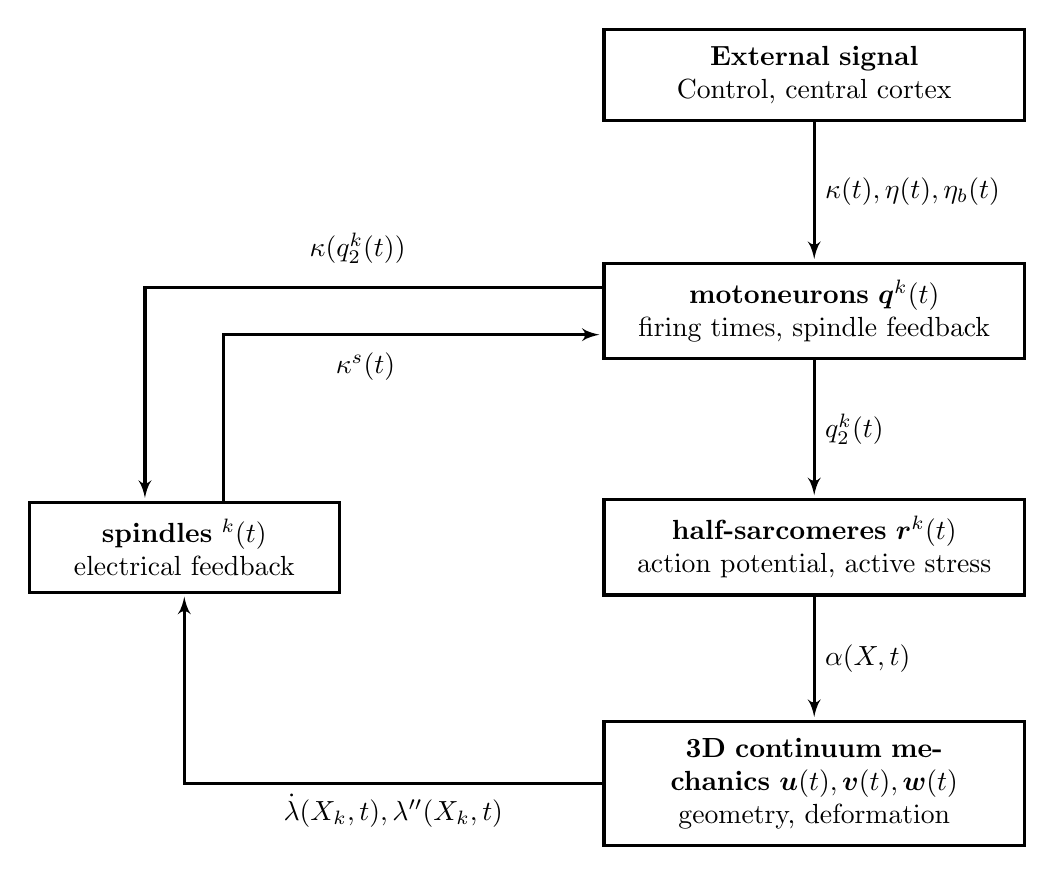
\begin{tikzpicture}[auto,%
            block_assign/.style ={rectangle, draw=black, very thick, fill=white,%
            text width=10em, text centered, minimum height=3em, inner sep=6pt},%
            block_big/.style ={rectangle, draw=black, very thick, fill=white,%
            text width=14em, text centered, minimum height=3em, inner sep=6pt},%
            block_dashed/.style ={rectangle, draw=black, very thick, fill=white,%
            text width=10em, text centered, minimum height=3em, inner sep=6pt},%
        ]%
        \tikzstyle{stateEdgePortion} = [black, very thick, -latex', shorten >=1pt];
        \tikzstyle{stateEdge} = [stateEdgePortion];
        \tikzstyle{edgeLabel} = [pos=0.5, text centered];
        \tikzstyle{edgeLabelLow} = [pos=0.25, text centered];
        \tikzstyle{edgeLabelHigh} = [pos=0.25, text centered];
        \tikzstyle{line} = [draw, black, very thick, -latex', shorten >=1pt]];
        \tikzstyle{sline} = [draw, black, very thick];
        \tikzstyle{dline} = [draw, black, dashed, very thick, -latex', shorten >=1pt]];
        \tikzstyle{doublearrow} = [draw, black, very thick, <->, -latex', shorten >=1pt, shorten <=5pt, >=stealth]];
%        \tikzstyle{doubledline} = [draw, black, dashed, very thick, <->, -latex', shorten >=1pt, shorten <=5pt, >=stealth]];
        \node [block_big] (neuro)  {{\bf motoneurons} $\vq^k(t)$\\firing times, spindle feedback};%
        \node [block_big, below of=neuro, node distance=30mm] (cell)  {{\bf half-sarcomeres $\vr^k(t)$}\\ action potential, active stress};%
        \node [block_big, above of=neuro, node distance=30mm] (ext)  {{\bf External signal}\\ Control, central cortex};%
        \node [block_dashed, left of=cell, node distance=80mm] (spindle)  {{\bf spindles $\vs^k(t)$} \\ electrical feedback};%
        \node [block_big, below of=cell, node distance=30mm] (mechanics)  {{\bf 3D continuum mechanics $\vu(t),\vv(t),\vw(t)$} \\ geometry, deformation};%
        \path [line] (neuro) -- (cell) node[edgeLabel]{$q^k_2(t)$};
        \draw (cell.south) edge[stateEdge] node[edgeLabel]{$\alpha(X,t)$} (mechanics.north);
        \path [line] (mechanics) -| (spindle) node[edgeLabelHigh]{$\dla(X_k,t),\la''(X_k,t)$};
    	\path [line] ($(neuro.west) + (0,0.3)$) -| ($(spindle.north) + (-0.5,0)$);
    	\path [line] ($(spindle.north) + (0.5,0)$) |- ($(neuro.west) + (0,-0.3)$);
    	\path [line] (ext) -- (neuro.north) node[edgeLabel] {$\kappa(t),\eta(t),\eta_b(t)$}; 
      	\node at (-5.7,-0.7) {$\kappa^s(t)$};
    	\node at (-5.8,0.8) {$\kappa(q^k_2(t))$};
    \end{tikzpicture}%
    \end{center}%
    \caption{Illustration of model connections and interaction}
    \label{fig:modelconn}
\end{figure}

\subsubsection{Motoneuron to Sarcomere}
The motoneuron soma signals $q^k_2(t)$ are used to provide activation spikes for the $k$-th sarcomere.
As the sarcomere model merely reacts to high spikes, the motoneuron output is scaled by a nonlinear function $\gamma$ to emphasize high peaks.
Essentially, the small signals are multiplied by a small factor $\beta_m = 0.3$, and the high signals are intensified by $\beta_M = 7$.
The transition from low to high factor is realized by a smooth Gaussian,
where we choose a threshold signal of $q_M = 40$ to pinpoint the signal from which on the $\beta_M$ factor is applied:
\begin{align}
	\gamma(q) &:= \begin{cases}
		\beta_m + e^{-(q-q_M)^2/150}(\beta_M-\beta_m), & 0 < q < q_M\\
		\beta_M & q \geq q_M,
	\end{cases}
\end{align}
Figure \ref{MSLink} illustrates the 
\begin{figure}[!ht]
	\centering
	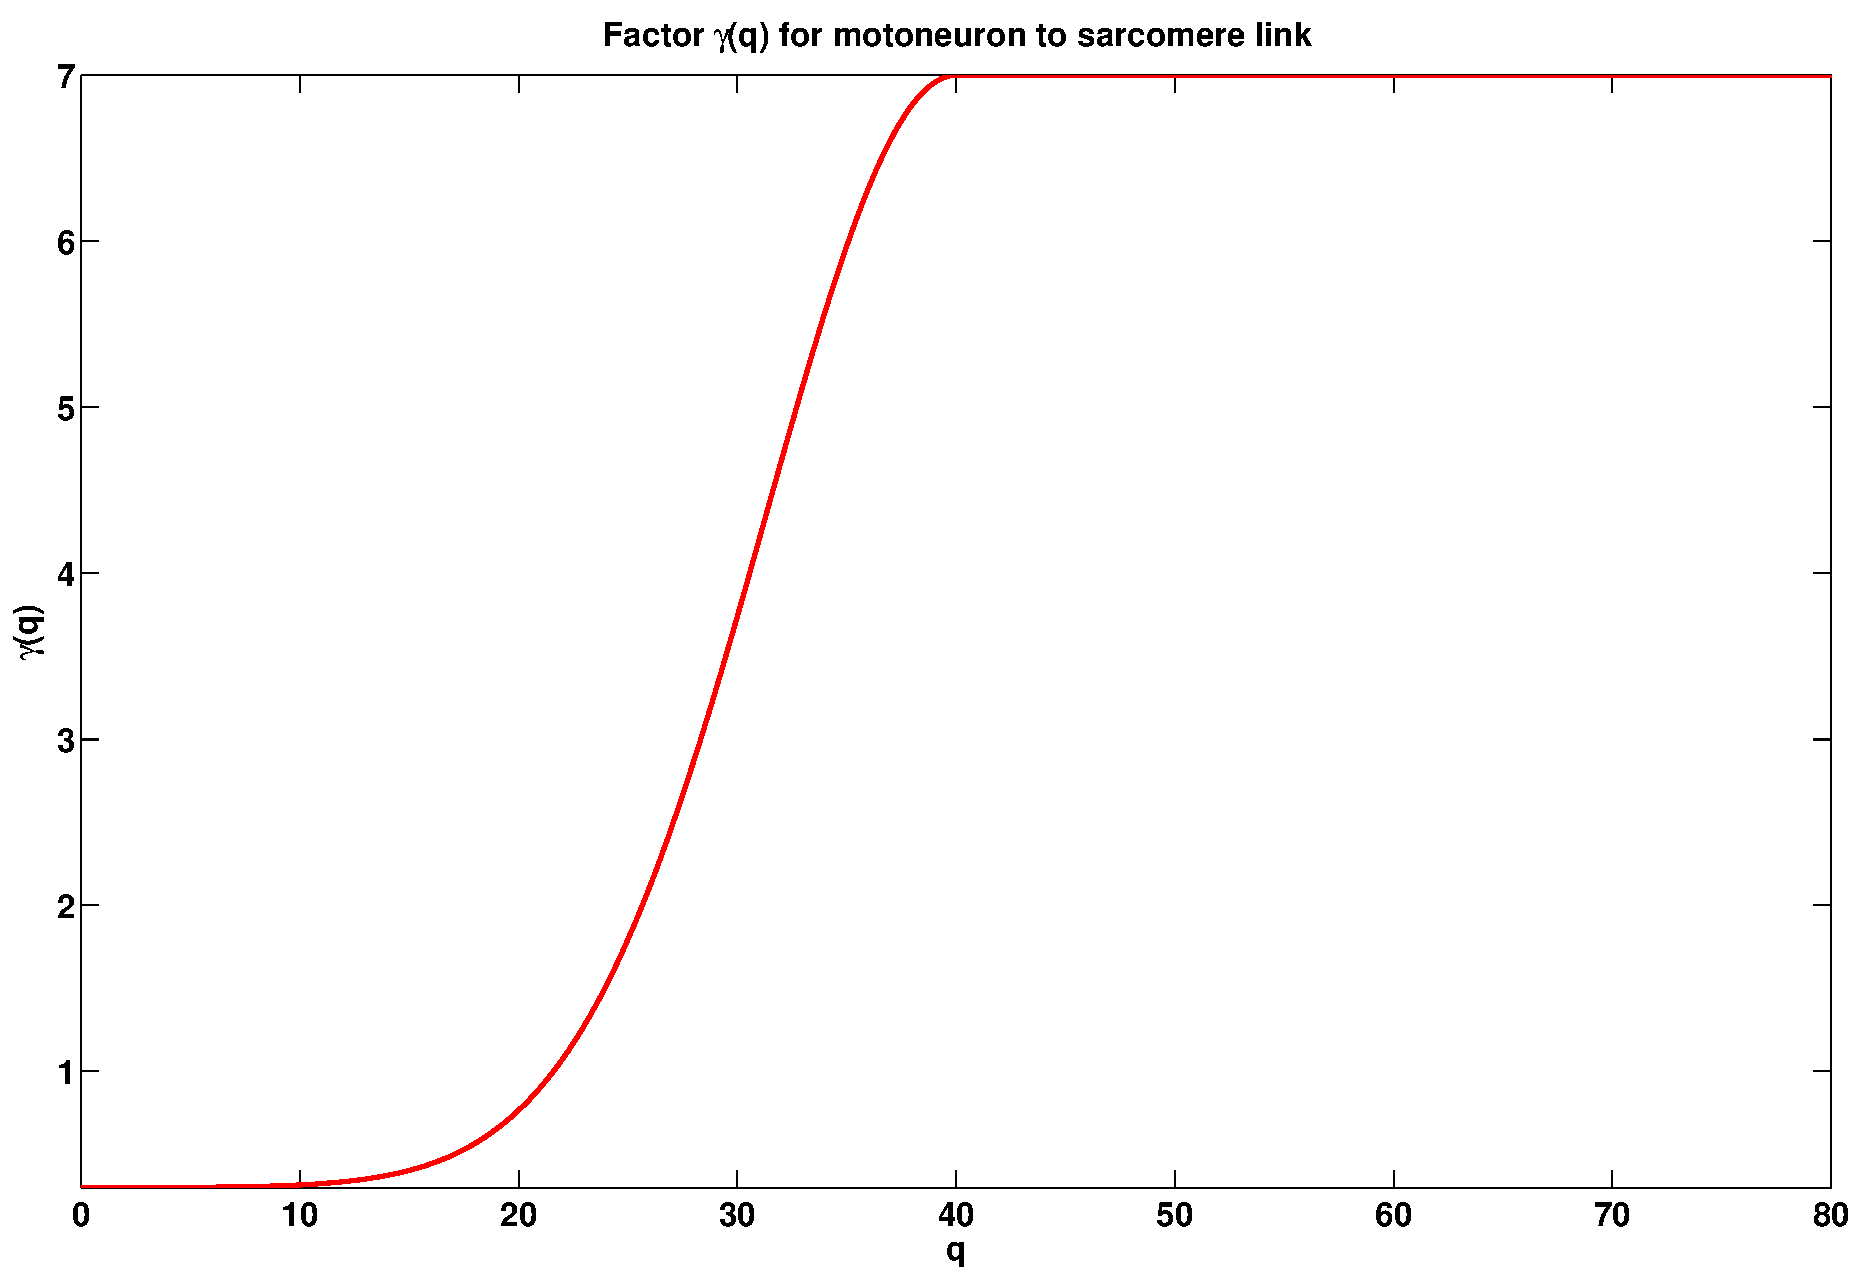
\includegraphics[width=\single]{moto_sarco_link_factor.pdf}
	\caption{Amplification factor for motoneuron signals}
	\label{fig:MSLink}
\end{figure}
Taking into account division by sarcomere model constants, the sarcomere models now read as
\begin{align}
	{\vr'}^k(t) &= \fsa(\vr^k(t),\tau_k) + \ve_1 \frac{\gamma(q_2^k(t))}{\csa_1(\tau_k)}q_2^k(t),\label{def:sarcosys_plus_moto}
\end{align}
where $\ve_1 \in \R^{56}$ denotes the first unit vector, i.e. the signal is added to the first component of the sarcomere models.

\subsubsection{Sarcomere to Mechanics}
The sarcomere model component $r_{53}^k(t)$ is an indicator for the currently developed force in the muscle fibre.
\fix{hier das modell aus der diss erwähnen mit fasern und diffusion + erläuterung}
Within the mechanics FE-framework, this can be transformed to active stress $\alpha(X,t)$ in $\vSf$ by weighting of all $\mups$ force signals at spatial locations.
Hence, we make the ansatz
\begin{align}
	\alpha(X,t) = \sum\limits_{k=1}^\mups w_k(X)\frac{r^k_{53}(t)-r^k_0}{r^k_M}.\label{def:alpha}
\end{align}
Here, we introduce weight functions $w_k(X)$ for the fibre forces satisfying $\sum w_k(X) = 1 \fo X$.
Further, the constants $r_0^k$ denote the base-line level of the $53$rd component and
$r^k_M\in\R$ are the maximum forces for each motorunit (i.e. $\tau_k$), determined by a long-time simulation of each sarcomere model using an
artificial $60Hz$ stimulation.
This ensures that $\alpha(X,t) \in [0,1] \fo X,t$. 

\subsubsection{Mechanics to Spindle}
According to \ref{def:spindlesys}, the spindle models use two external inputs:
The current change rate $\dla$ of fibre stretch and the motoneuron frequency $\kappa(t)$, where the latter will be discussed in Section
\ref{subsec:moto_spindle}.
As the fibre stretch is a local property of the continuum, we fix $\mups$ spindle locations $X_k\in\Omega$ and simply observe $\dla(X_k,t)$ to obtain the second
argument of the $k$-th spindle dynamics $\fsp$.
We recall the definition \eqref{def:fibrestretch} and observe 
\begin{align}
	\dla(X,t) &= \d{}{t}\no{\vF(X,t)\va_0(X)} = \frac{(\vF(X,t)\va_0(X))^T}{\no{\vF(X,t)\va_0(X)}}\d{}{t}\vF(X,t)\va_0(X)\nonumber\\
	  &= \frac{1}{\la(X,t)}\va_0(X)^T\vF(X,t)^T\dot{\vF}(X,t)\va_0(X).\label{eq:dlambda}
\end{align}
Hence, if the $X_k$ are chosen among the set of all elements' Gauss integration points, quantities to compute $\dla$ are readily available during mechanics evaluation.

\subsubsection{Spindle to Motoneuron}
According to \cite{Mileusnic2006}, the spindle model has two algebraic scalar quantities called \e{primary} and \e{secondary afferents},
denoted by $\theta_p(\vs^k(t))$ and $\theta_s(\vs^k(t))$, respectively.
These afferents describe the firing frequency in [pps] of the spindle dendrites leading back into the motoneuron pool.
In a muscle, all spindles are connected to the entirety of the motoneuron pool \fix{ref?}, which will be modeled via averaging of all $\mups$ spindle's afferent outputs.
This gives a \e{mean spindle activation} of
\begin{align}
	\kappa^s(t) &:= \frac{1}{\mups}\sumjmups w_p\theta_p(\vs^j(t)) + w_s\theta_s(\vs^j(t))
\end{align}
which is added to the change rate of each motoneuron's soma alike the external mean current:
\begin{align}
	\dot{\vq}(t) &= \fmo(\vq(t),\tau) + \ve_2(\kappa(t) + \kappa^s(t))\eta(t,\tau) + \ve_2\eta_b(t).\label{def:motosys_plus_spindle}
\end{align}    
% [6{:}8] , where the \ML-like notation indicates which components of the spindle states $\vs$ are used as arguments.

\subsubsection{Motoneuron to Spindle}\label{subsec:moto_spindle}
In order to provide the Spindle model with the current motoneuron frequency, the discrete signal $s_n := q^k_2(t_n)$ at times $t_n, t_1 < t_2 < t_3 \ldots$ needs to be converted to
a frequency $\nu_n$.
Essentially, the last $W \in\N$ peaks are tracked and the frequency is determined by the time elapsed between the last $W$ peaks.    
This is done by a simple automata described in Figure \ref{fig:FD}, where we have two thresholds $p^+,p^-$ denoting the start and end of a peak, respectively.
\begin{figure}[!ht]
    \centering
	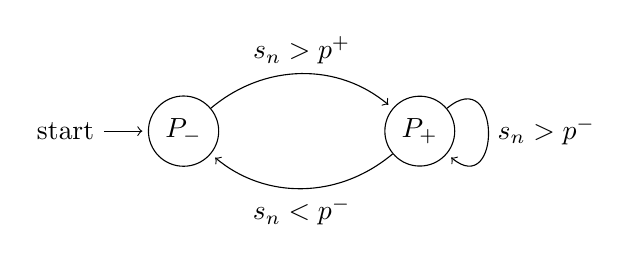
\begin{tikzpicture}[shorten >= 2pt, node distance=2cm, auto]
		\node (S) at (-.5,0) {start};
		\node[state] (poff) at (1,0) {$P_-$};
		\node[state] (pon) at (4,0) {$P_+$};
		\path[->] (S) edge node {} (poff)
				  (poff) edge[out=40,in=140] node[above] {$s_n > p^+$} (pon)
				  (pon) edge[out=40,in=320,looseness=4] node[right] {$s_n > p^-$} (pon)
				  (pon) edge[out=220,in=320] node[below] {$s_n < p^-$} (poff);
	\end{tikzpicture}
    \caption{Frequency-detection automata}\label{fig:FD}
\end{figure}
Whenever the transition from $P_-$ to $P_+$ is done, the ``peak counter'' $k$ (starting from $k=0$) is increased by one and the current time $t_n$ is stored via $t^p_k = t_n$.
Then the frequency sequence is then given by
\begin{align}
	\nu_n &:= \begin{cases}
		\frac{W}{t_n - t^p_{k-W}} & k \geq W,\\
		0 & k < W.
	\end{cases}\label{def:FD_freq}
\end{align}
As the detector essentially computes a local average over $W$ peaks, a larger ``window size'' $W$ improves accuracy with respect to a noisy signal,
while a smaller $W$ renders the detector more sensitive to quick frequency changes.
In our applications $W=3$ or $W=4$ turned out to be appropriate choices.

Alternatively, as the frequency detector has a window-size dependent delay, the resulting motoneuron frequency for any given fibre type and 
mean current can be approximated by a machine learning approach \cite{Wirtz2013a}.
Essentially, collected frequencies $\nu_l$ for parameter pairs $(\tau_l,\kappa_l), l = 1\ldots L$ are used as training data
and the approximation is build to have $\nu \approx \tnu(\tau,\kappa)$ for a new, previously unknown pair $(\tau,\kappa)$ and actual frequency $\nu$.
The left image of Figure \ref{fig:motofreq} shows the raw frequency data measured by the frequency detector described above for a sufficiently long run-time using a suitable training set.
The data is then smoothed by multiple 2D-convolution and learned by the VKOGA algorithm using Wendland kernels \cite{Wirtz2013a, Wirtz2013, Wendland2005}.
Figure \ref{fig:motofreq} shows the smoothed frequency responses and the learned surface.
\begin{figure}[!ht]
	\centering
	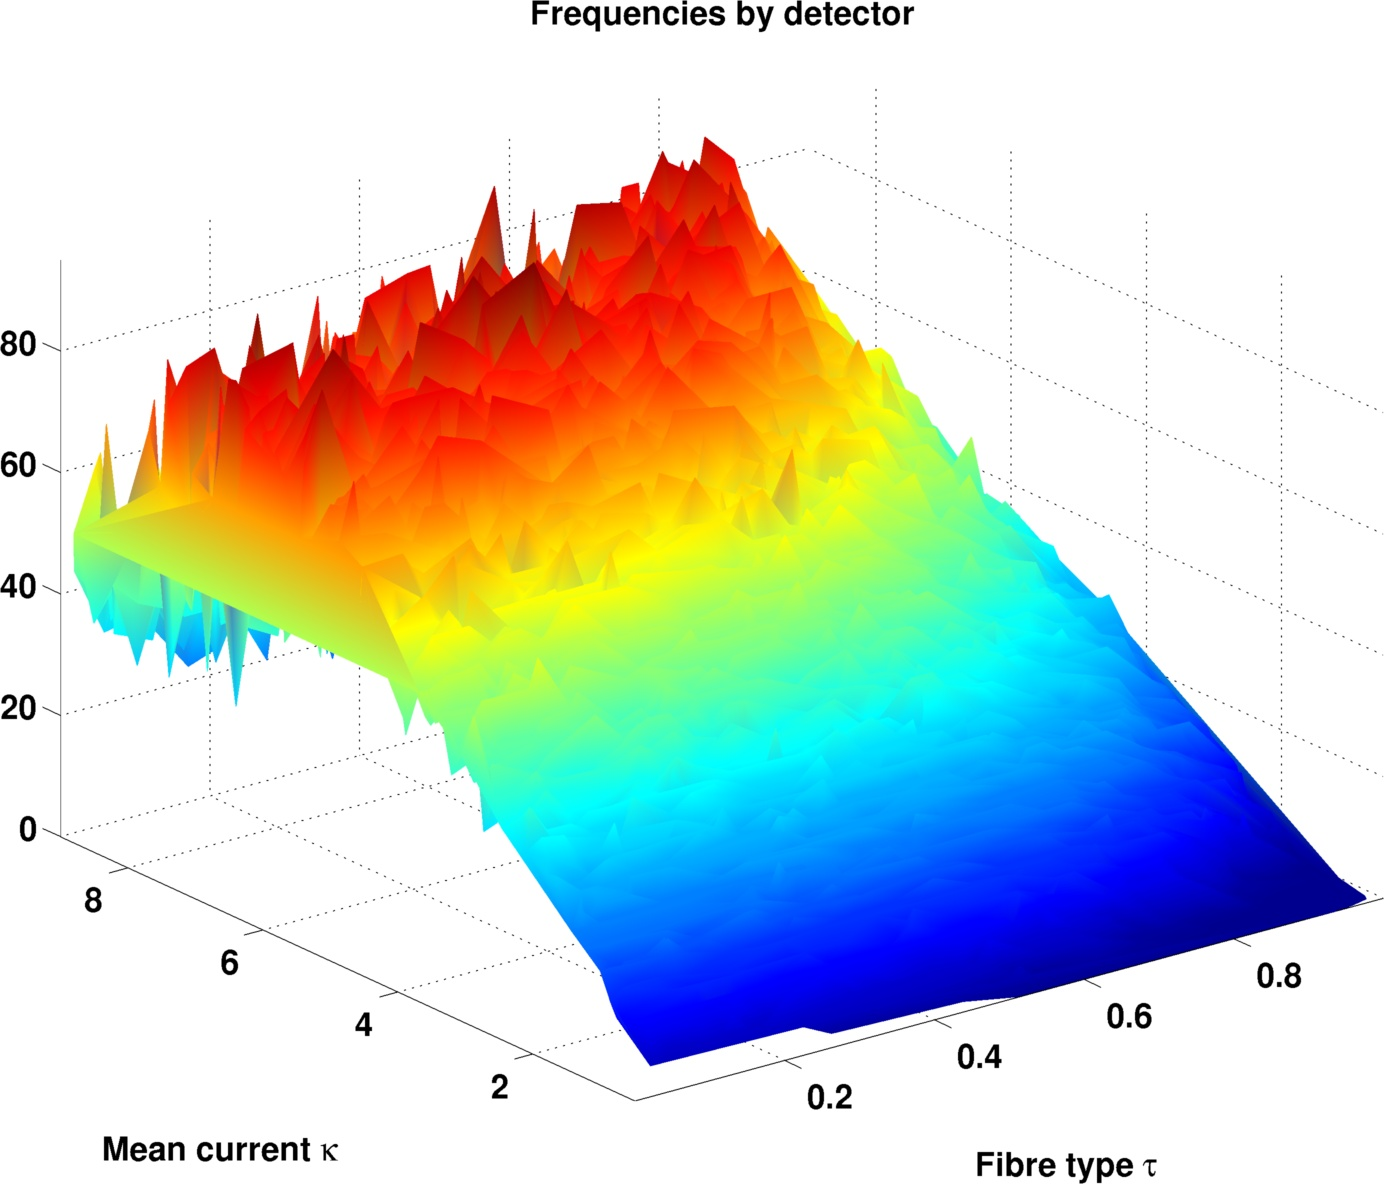
\includegraphics[width=\third]{freq_raw_data}
	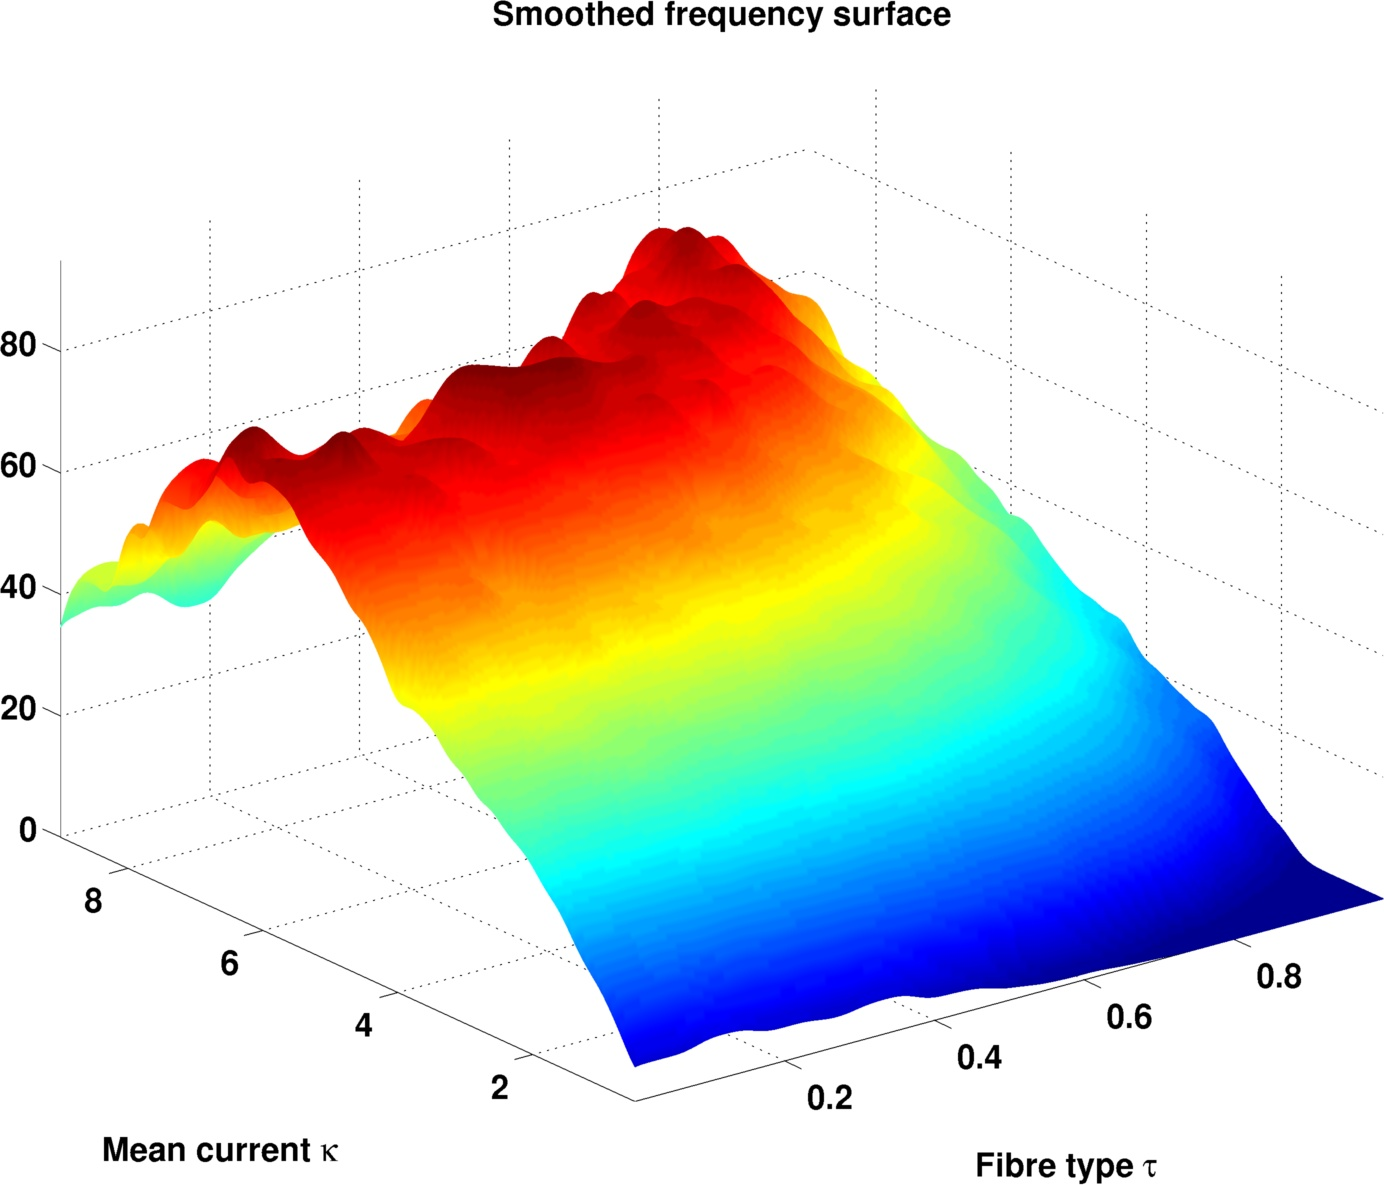
\includegraphics[width=\third]{freq_smoothed}
	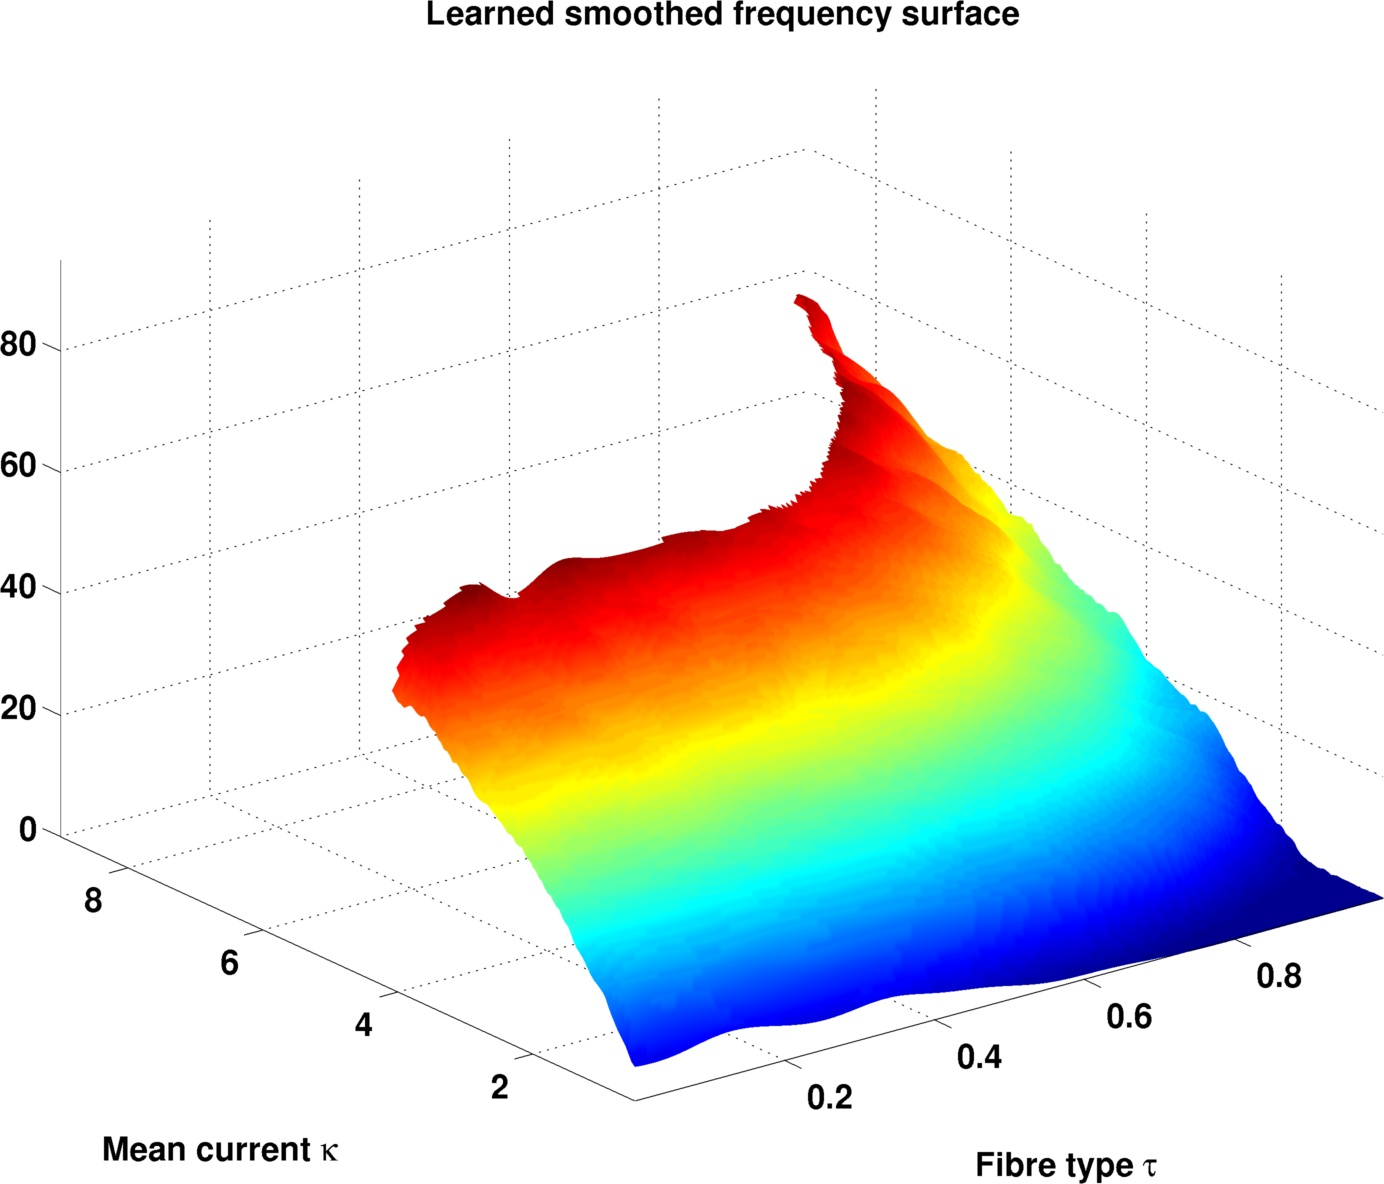
\includegraphics[width=\third]{freq_approx}
	\caption{Frequency response of Motoneurons in Hz for different fibre types $\tau$ and mean currents $\kappa$.
	Left: Raw data, center: smoothed data, right: Learned response surface (cut to the region of valid inputs, see Section \ref{sec:motoneuron})}
	\label{fig:motofreq}
\end{figure}
Mathematically, the VKOGA yields a kernel expansion
\begin{align}
	\tnu(\vz) &= \suml{j=1}{C}c_j\Phi(\vz,\vz_j), & c_j &\in \R,  & \vz_j\in\R^2. 
\end{align}
Here, the kernel $\Phi$ is a Wendland kernel given by
\begin{align}
	\Phi(\vz,\tilde{\vz}) &= \phi\left(\frac{\noG{\vz-\tilde{\vz}}}{\gamma}\right), & \phi(r) &= (1-r)^{l+k}_+p(r),\\
	p(r) &= \frac{1}{3}(l^2 + 4l + 3)r^2 + (l + 2)r + 1, & l &:= \lfloor d/2\rfloor + k + 1.
\end{align}
where we used $k=d=2$.
Here, $k$ is a hyperparameter for \e{smoothness} in the sense of $\Phi\in C^{2k}(\Omega)$ if $\Omega \subseteq \R^{\hat{d}}, \hat{d}\leq d$, see \cite{Wendland2005}.

With this, instead of using \eqref{def:FD_freq}, one can obtain the current $k$-th motoneuron frequency as $\tnu(\tau_k,\kappa)$ for given mean current $\kappa$.

\subsubsection{Model parameters}
\begin{table}[!ht]
	\begin{tabular}{l|l|l}
		Name & Value & Context\\\hline
		$\beta_m$ & 0.3 & Moto-Sarco link min factor\\
		$\beta_M$ & 7 & Moto-Sarco link max factor\\
		$q_M$ & 40 & Moto-Sarco link max factor signal\\
		$w_p$ & 0.002 & Primary afferent weight\\
		$w_s$ & 0.002 & Secondary afferent weight\\
		$p^+$ & 40 & Frequency detector ``peak on'' threshold\\
		$p^-$ & 15 & Frequency detector ``peak off'' threshold\\
		$W$ & 3-4 & Frequency detector peak window size
	\end{tabular}
	\caption{Model-related parameters}\label{tab:params}
\end{table}
\begin{table}[!ht]
	\begin{tabular}{l|ll}
		Name & Context\\\hline
		$r^k_M$ & Maximum force response of single sarcomere at constant, full activation ($60Hz$)\\
		$r^k_0$ & Base-line or minimum force response of the $k$-th sarcomere 
	\end{tabular}
	\caption{Experimentally determined quantities}\label{tab:params}
\end{table}
\begin{table}[!ht]
	\begin{tabular}{l|ll}
		Name &  Context\\\hline
		$w_k$ & Weights for fibre forces at each Gauss point  
	\end{tabular}
	\caption{Model design variables}\label{tab:params}
\end{table}

\section{Overall dynamical system}
In this section we detail the numerical implementation of the overall connected model as system of ODEs.
The muscle activation introduced in Section \ref{sec:active_force} now is computed using the sarcomere states $\vr^k$.
This renders the stress tensor \eqref{def:completeP} and hence the operator $K$ from \eqref{def:Kop} dependent of $\vr^1(t),\ldots,\vr^\mups(t)$,
so we write $K(\vu(t),\vw(t),\vr^1(t),\ldots,\vr^\mups(t))$.
Moreover, the motoneurons \eqref{def:motosys} receive feedback from all spindles via $\kappa^s(\vs^1(t),\ldots,\vs^\mups(t))$.
%As each sarcomere is linked to its motoneuron, the sarcomere dynamics \eqref{def:sarcosys} now read as $\fsa(\vr^k(t),\tau_k,\vq^k(t))$.
The spindles \ref{def:spindlesys} receive lambda stretch information $\dla(X_k,t)$ from the mechanics model at locations $X_k$.
Recalling \eqref{eq:Fdependencyrewrite} and the substitution $\vv(t) = \vu'(t)$ from Section \ref{sec:odeform} we see that similarly
\begin{align}
	\dot{\vF}(X,t) &= \sumi \vc'_i(t)\otimes \nabla\varphi_i(X) = \sumi \vv[i](t)\otimes \nabla\varphi_i(X) =: \dot{\vF}(X,\vv(t)).\label{eq:Fdotdependencyrewrite}
\end{align}
Hence, by virtue of \eqref{eq:dlambda}, we see that $\dla(X,t) =: \dla(X,\vu(t),\vv(t))$, which finally gives $\fsp(\vs^k(t),\vu(t),\vv(t))$.

Finally, using the above, \eqref{def:motosys_plus_spindle} and \eqref{def:sarcosys_plus_moto}, the overall system \eqref{def:mainsys} can be extended to
\begin{align}%\label{def:mainsys_full}
	\dot{\vu}(t) &= \vv(t)\\
	\vM\dot{\vv}(t) &= -K(\vu(t),\vw(t),\vr^1(t),\ldots,\vr^\mups(t)) - \vD\vv(t)\\
		& \vdots\nonumber\\
	\dot{\vq}^k(t) &= \fmo(\vq^k(t),\tau_k) + \ve_2^9(\kappa(t) + \kappa^s(\vs^1(t),\ldots,\vs^\mups(t)))\eta(t,\tau) + \ve_2^9\eta_b(t)\\
		 & \vdots\nonumber\\
	\dot{\vr}^k(t) &= \fsa(\vr^k(t),\tau_k) + \ve^{56}_1 \frac{\gamma(q_2^k(t))}{\csa_1(\tau_1)}q_2^k(t)\\
		& \vdots\nonumber\\
	\dot{\vs}^k(t) &= \fsp(\vs^k(t),\vu(t),\vv(t))\\
		& \vdots\nonumber\\
% 	\dot{\vq}^1(t) &= \fmo(\vq^1(t),\tau_1) + \ve_2(\kappa(t) + \kappa^s(\vs^1(t),\ldots,\vs^\mups(t)))\eta(t,\tau) + \ve_2\eta_b(t)\\
% 		\vdots &= \vdots\nonumber\\
% 	\dot{\vq}^\mups(t) &= \fmo(\vq^\mups(t),\tau_\mups) + \ve_2(\kappa(t) + \kappa^s(\vs^1(t),\ldots,\vs^\mups(t)))\eta(t,\tau) + \ve_2\eta_b(t)\\
% 	\dot{\vr^1}(t) &= \fsa(\vr^1(t),\tau_1) + \ve_1 \frac{\gamma(\vq_2^1(t))}{\csa_1(\tau_1)}\vq_2^1(t)\\
% 		\vdots &= \vdots\nonumber\\
% 	\dot{\vr^\mups}(t) &= \fsa(\vr^\mups(t),\tau_\mups) + \ve_1 \frac{\gamma(\vq_2^\mups(t))}{\csa_1(\tau_\mups)}\vq_2^\mups(t)\\
% 	\dot{\vs^1}(t) &= \fsp(\vs^1(t),\vu(t),\vv(t))\\
% 		\vdots &= \vdots\nonumber\\
% 	\dot{\vs^\mups}(t) &= \fsp(\vs^\mups(t),\vu(t),\vv(t))\\
	\text{s.t.}\quad \vg(\vu(t))		&= \vnull.
\end{align}

\subsection{Derivation of $\nabla_{\vr^k}K(\vu(t),\vw(t),\vr^1(t),\ldots,\vr^\mups(t))$}
For any $k = 1\ldots\mups, j=1\ldots N$ we have similar to \eqref{def:dKduji}
\begin{align}
	\d{K[j]}{r^k_i}(\vu,\vw,\vr^1,\ldots,\vr^\mups) &= \sumvk\sumgp w_p \d{\vPnl}{r^k_i}(\pmp,\vu,\vw,\ldots,\vr^k,\ldots) \dNjmp\jmp\\
	\d{\vPnl}{r^k_i}(\ldots,\vr^k,\ldots) & \re{def:completeP} \d{}{r^k_i} g(\la(\pmp,\vu),\dla(\pmp,\vu,\vv),\alpha(\pmp,\vr^1,\ldots,\vr^\mups))\nonumber\\
	&\qquad\cdot\vF(\pmp,\vu)\va_0(\pmp)\otimes\va_0(\pmp)\\
	&= \d{g}{\alpha}(\la(\pmp,\vu),\dla(\pmp,\vu,\vv),\alpha)\d{\alpha}{r^k_i}(\pmp,\vr^1,\ldots,\vr^\mups)\nonumber\\
	&\qquad\cdot\vF(\pmp,\vu)\va_0(\pmp)\otimes\va_0(\pmp)\\
	\d{g}{\alpha}(\la,\dla,\alpha) &\re{def:g} \frac{p^{max}}{\la}f_l(\la)f_v(\dla)\\
	\d{\alpha}{r^k_i}(\pmp,\vr^1,\ldots,\vr^\mups) &\re{def:alpha} \d{}{r^k_i}\sum\limits_{l=1}^\mups w_l(\pmp)\frac{r^l_{53}(t)-r^l_0}{r^l_M} = \begin{cases}
		\frac{w_k(\pmp)}{r^k_M} & i=53\\
		0 & \text{else}
	\end{cases}
\end{align}
\begin{align}	
	\Rightarrow\d{K[j]}{r^k_{53}} &= \sumvk\sumgp w_p \Biggl(\frac{p^{max}}{\la(\pmp,\vu)}f_l(\la(\pmp,\vu))f_v(\dla(\pmp,\vu,\vv))\frac{w_k(\pmp)}{r^k_M}\nonumber\\
	&\qquad \cdot \vF(\pmp,\vu)\va_0(\pmp)\otimes\va_0(\pmp)\dNjmp\jmp\Biggr),\\
	\d{K[j]}{r^k_i} &= 0 \qquad i \neq 53
\end{align}

\subsection{Moto to Sarco Jacobian}
\begin{align}
	\d{}{q_2^k}\dot{r}_1^k(\vr^k,\tau_k) &= \d{}{q_2^k}\frac{\gamma(q_2^k)}{\csa_1(\tau_k)}q_2^k = \frac{\gamma(q_2^k)}{\csa_1(\tau_k)} + \frac{q_2^k}{\csa_1(\tau_k)}\d{}{q_2^k}\gamma(q_2^k)\\
	&=  \frac{\gamma(q_2^k)}{\csa_1(\tau_k)} - \frac{q_2^k(q_2^k-q_M)}{\csa_1(\tau_k)75}e^{-(q_2^k-q_M)^2/150}(\beta_M-\beta_m)
\end{align}

\subsection{Spindle to Moto}
\begin{align}
	\d{}{s^k_i}\dot{\vq}(t) &= \d{}{s^k_i}\ve_2(\kappa(t) + \kappa^s(\vs^1,\ldots,\vs^\mups))\eta(t,\tau)\\
	&= \ve_2\eta(t,\tau)\d{}{s^k_i}\kappa^s(\vs^1,\ldots,\vs^\mups)\\
	&= \ve_2\frac{\eta(t,\tau)}{\mups}\d{}{s^k_i}\sumjmups w_p\theta_p(\vs^j) + w_s\theta_s(\vs^j)\\
	&= \ve_2\frac{\eta(t,\tau)}{\mups}\left(w_p\d{}{s^k_i}\theta_p(\vs^k) + w_s\d{}{s^k_i}\theta_s(\vs^k)\right)
\end{align}

\subsection{Spindle via learned Frequency}
If the learned frequency $\tnu$ is used, the spindle link via the motoneuron leads to an immediate feedback for the spindle dynamics as then
\begin{align}
	\dot{\vs}^k(t) &= \fsp(\vs^k(t),\dla(t),\tnu(t))\\
	&= \fsp(\vs^k(t),\dla(t),\tnu(\tau_k,\kappa(t) + \kappa^s(\vs^1(t),\ldots,\vs^\mups(t))))
\end{align}
Hence we get
\begin{align}
	\d{}{s_i^j}\fsp(\vs^k,\dla,\tnu(\vs^1,\ldots,\vs^\mups)) &= \delta_{jk}\frac{\partial_1}{\partial s_i^j}\fsp(\vs^k,\dla,\tnu)
	 + \frac{\partial_3}{\partial s_i^j}\fsp(\vs^k,\dla,\tnu(\vs^1,\ldots,\vs^\mups))\\
	\frac{\partial_3}{\partial s_i^j}\fsp(\vs^k,\dla,\tnu(\vs^1,\ldots,\vs^\mups))
	&= \d{}{\tnu}\fsp(\vs^k,\dla,\tnu)\d{}{\kappa}\tnu(\tau,\kappa)\d{}{s_i^j}\kappa^s(\vs^1,\ldots,\vs^\mups)
\end{align}
\begin{align}
	[\ldots]&= \d{}{\tnu}\fsp(\vs^k,\dla,\tnu)\suml{l=1}{C}c_l\d{}{\kappa}\Phi((\tau_k,\kappa),\vz_l)
	\frac{1}{\mups}\left(w_p\d{}{s^j_i}\theta_p(\vs^j) + w_s\d{}{s^j_i}\theta_s(\vs^j)\right)
\end{align}

\subsection{Mechanics to Spindle}
For $k=1\ldots\mups, j = 1\ldots N, i=1\ldots3$ we have
\begin{align}
	\d{}{\vu[j]_i}\fsp(\vs^k,\dla(X,\vu,\vv),\nu) &= \d{}{\dla}\fsp(\vs^k,\dla,\nu)\d{}{\vu[j]_i}\dla(X,\vu,\vv)\\
	\d{}{\vu[j]_i}\dla(X,\vu,\vv) &\re{eq:dlambda} \d{}{\vu[j]_i}\frac{1}{\la(X,\vu)}\va_0(X)^T\vF(X,\vu)^T\dot{\vF}(X,\vv)\va_0(X)
\end{align}
\begin{align*}
   \d{}{\vu[j]_i} [\ldots] &= \d{}{\vu[j]_i}\left(\frac{1}{\la(X,\vu)}\right)\va_0(X)^T\vF(X,\vu)^T\dot{\vF}(X,\vv)\va_0(X)\\
   &\quad+ \frac{1}{\la(X,\vu)}\d{}{\vu[j]_i}\va_0(X)^T\dot{\vF}(X,\vv)^T\vF(X,\vu)\va_0(X)\\
   &= -\frac{1}{\la(X,\vu)^2}\d{}{\vu[j]_i}\Bigl(\la(X,\vu)\Bigr)\va_0(X)^T\vF(X,\vu)^T\dot{\vF}(X,\vv)\va_0(X)\\
   &\quad+ \frac{1}{\la(X,\vu)}\va_0(X)^T\dot{\vF}(X,\vv)^T\vU_i^j\va_0(X)\\
   &\re{eq:dlamdvu} -\frac{1}{\la(X,\vu)^3}\va_0(X)^T\vF(X,\vu)^T\Bigl(\vU_i^j+\dot{\vF}(X,\vv)\Bigr)\va_0(X)\\
   &\quad+ \frac{1}{\la(X,\vu)}\va_0(X)^T\dot{\vF}(X,\vv)^T\vU_i^j\va_0(X)
\end{align*}
\begin{align}
	\d{}{\vv[j]_i}\fsp(\vs^k,\dla(X,\vu,\vv),\nu) &= \d{}{\dla}\fsp(\vs^k,\dla,\nu)\d{}{\vv[j]_i}\dla(X,\vu,\vv)\\
	\d{}{\vv[j]_i}\dla(X,\vu,\vv) &\re{eq:dlambda} \d{}{\vv[j]_i}\frac{1}{\la(X,\vu)}\va_0(X)^T\vF(X,\vu)^T\dot{\vF}(X,\vv)\va_0(X)\\
		&=\frac{1}{\la(X,\vu)}\va_0(X)^T\vF(X,\vu)^T\d{}{\vv[j]_i}\dot{\vF}(X,\vv)\va_0(X)\\
		&\re{eq:Fdotdependencyrewrite}\frac{1}{\la(X,\vu)}\va_0(X)^T\vF(X,\vu)^T\vU^j_i\va_0(X)
\end{align}

\subsection{Model connectivity}
The above partial derivatives constitute the overall system Jacobian matrix.
Figure \ref{fig:jacpattern} illustrates the Jacobian sparsity pattern for an example geometry with $18$ Taylor-Hood elements and $\mups=6$ motorunits and spindles.
\begin{figure}[!ht]
	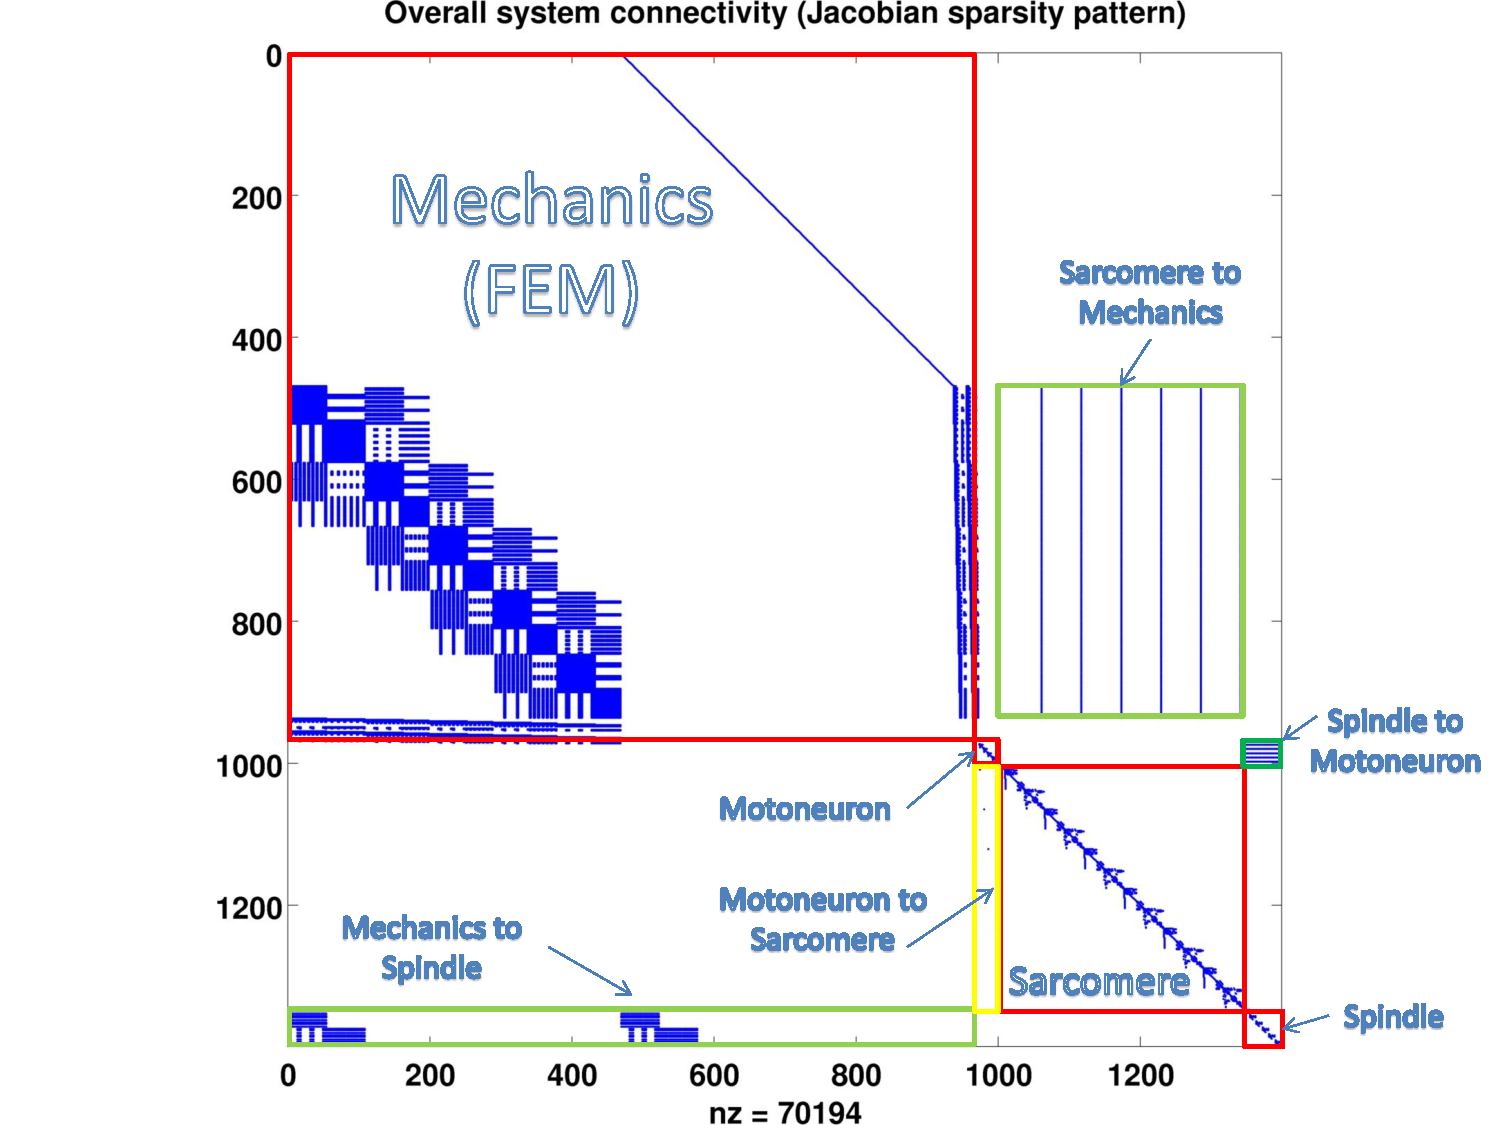
\includegraphics[width=\textwidth]{sparsity_pattern}
	\caption{Jacobian sparsity pattern}
	\label{fig:jacpattern}
\end{figure}


\newpage
\section{Appendix, additional derivations}

\subsection{Calculation of $\nabla_{\Bc_m}\left\{\det \BF(X,t)\right\}$}
Calculation of the determinant:
\begin{align}
  \nabla_{\Bc_m}\left\{\det \BF(X,t)\right\}
  &=\nabla_{\Bc_m}\left\{\det \left( \sumlim{i=1}{N}{\Bc_i(t) \otimes \nabla \varphi_i(X)} \right) \right\} \nonumber\\
  &=\nabla_{\Bc_m}\left\{\det \left( \sumlim{i=1}{N}{
      \begin{bmatrix}
        c_{i1} \varphi_{i,1}  & c_{i1} \varphi_{i,2}  & c_{i1} \varphi_{i,3} \\
        c_{i2} \varphi_{i,1}  & c_{i2} \varphi_{i,2}  & c_{i2} \varphi_{i,3} \\
        c_{i3} \varphi_{i,1}  & c_{i3} \varphi_{i,2}  & c_{i3} \varphi_{i,3}
      \end{bmatrix}
    } \right) \right\} \nonumber\\
  &=\nabla_{\Bc_m}\Bigg\{
      \left( \sumlim{i=1}{N}{c_{i1}\varphi_{i,1}}\right) \left[
        \left( \sumlim{i=1}{N}{c_{i2}\varphi_{i,2}}\right) \left( \sumlim{i=1}{N}{c_{i3}\varphi_{i,3}}\right)
        - \left( \sumlim{i=1}{N}{c_{i2}\varphi_{i,3}}\right) \left( \sumlim{i=1}{N}{c_{i3}\varphi_{i,2}}\right)
      \right]
      \nonumber\\
      &\hspace{11.5mm} -\left( \sumlim{i=1}{N}{c_{i1}\varphi_{i,2}}\right) \left[
        \left( \sumlim{i=1}{N}{c_{i2}\varphi_{i,1}}\right) \left( \sumlim{i=1}{N}{c_{i3}\varphi_{i,3}}\right)
        - \left( \sumlim{i=1}{N}{c_{i2}\varphi_{i,3}}\right) \left( \sumlim{i=1}{N}{c_{i3}\varphi_{i,1}}\right)
      \right]
      \nonumber\\
      &\hspace{11.5mm} +\left( \sumlim{i=1}{N}{c_{i1}\varphi_{i,3}}\right) \left[
        \left( \sumlim{i=1}{N}{c_{i2}\varphi_{i,1}}\right) \left( \sumlim{i=1}{N}{c_{i3}\varphi_{i,2}}\right)
        - \left( \sumlim{i=1}{N}{c_{i2}\varphi_{i,2}}\right) \left( \sumlim{i=1}{N}{c_{i3}\varphi_{i,1}}\right)
      \right]
    \Bigg\}\nonumber\\
  &=\nabla_{\Bc_m}\Bigg\{
  \sumlim{i,j,k=1}{N}{c_{i1} \varphi_{i,1} \, c_{j2} \varphi_{j,2} \, c_{k3}\varphi_{k,3}}
    -\sumlim{i,j,k=1}{N}{c_{i1} \varphi_{i,1} \, c_{j2} \varphi_{j,3} \, c_{k3}\varphi_{k,2}}
    \nonumber\\
    &\hspace{11.5mm}-\sumlim{i,j,k=1}{N}{c_{i1} \varphi_{i,2} \, c_{j2} \varphi_{j,1} \, c_{k3}\varphi_{k,3}}
    +\sumlim{i,j,k=1}{N}{c_{i1} \varphi_{i,2} \, c_{j2} \varphi_{j,3} \, c_{k3}\varphi_{k,1}}
    \nonumber\\
    &\hspace{11.5mm}+\sumlim{i,j,k=1}{N}{c_{i1} \varphi_{i,3} \, c_{j2} \varphi_{j,1} \, c_{k3}\varphi_{k,2}}
    -\sumlim{i,j,k=1}{N}{c_{i1} \varphi_{i,3} \, c_{j2} \varphi_{j,2} \, c_{k3}\varphi_{k,1}} 
    \Bigg\}\nonumber\\
  &=\nabla_{\Bc_m}\Bigg\{
    \sumlim{i,j,k=1}{N}{
    c_{i1} c_{j2} c_{k3} (
      \varphi_{i,1} \varphi_{j,2} \varphi_{k,3}-\varphi_{i,1} \varphi_{j,3} \varphi_{k,2}-\varphi_{i,2} \varphi_{j,1} \varphi_{k,3}
      }\nonumber\\
      &\hspace{20mm}+\varphi_{i,2} \varphi_{j,3} \varphi_{k,1}+\varphi_{i,3} \varphi_{j,1} \varphi_{k,2}
      -\varphi_{i,3} \varphi_{j,2} \varphi_{k,1} )
    \Bigg\}\nonumber\\
  &=\nabla_{\Bc_m}\Bigg\{
      \sumlim{i,j,k=1}{N}{
      c_{i1} c_{j2} c_{k3} 
      \det  \begin{bmatrix}
              \varphi_{i,1} & \varphi_{i,2} & \varphi_{i,3} \\
              \varphi_{j,1} & \varphi_{j,2} & \varphi_{j,3} \\
              \varphi_{k,1} & \varphi_{k,2} & \varphi_{k,3}
            \end{bmatrix}
      }
    \Bigg\} \nonumber\\
  &=\nabla_{\Bc_m}\Bigg\{
      \sumlim{i,j,k=1}{N}{
      c_{i1}(t) c_{j2}(t) c_{k3}(t)
      \det \begin{bmatrix}
              \nabla \varphi_{i}(X) \\
              \nabla \varphi_{j}(X) \\
              \nabla \varphi_{k}(X)
            \end{bmatrix}
      }
    \Bigg\}
\end{align}
%
%-------
\newpage
%-------
%
Calculation of the gradient:
\begin{align}
  \nabla_{\Bc_m}\left\{\det \BF(X,t)\right\}
  &=\nabla_{\Bc_m}\Bigg\{
      \sumlim{i,j,k=1}{N}{
      c_{i1}(t) c_{j2}(t) c_{k3}(t)
      \det \begin{bmatrix}
              \nabla \varphi_{i}(X) \\
              \nabla \varphi_{j}(X) \\
              \nabla \varphi_{k}(X)
            \end{bmatrix}
      }
    \Bigg\} \nonumber\\
  &=\sumlim{i,j,k=1}{N}{\left(
      \begin{bmatrix}
        \delby{c_{i1}}{c_{m1}}c_{j2}c_{k3} + c_{i1} \cancel{\delby{c_{j2}}{c_{m1}}} c_{k3} 
          + c_{i1}c_{j2}\cancel{\delby{c_{k3}}{c_{m1}}} \\
        \cancel{\delby{c_{i1}}{c_{m2}}}c_{j2}c_{k3} + c_{i1} \delby{c_{j2}}{c_{m2}} c_{k3} 
          + c_{i1}c_{j2}\cancel{\delby{c_{k3}}{c_{m2}}} \\
        \cancel{\delby{c_{i1}}{c_{m3}}}c_{j2}c_{k3} + c_{i1} \cancel{\delby{c_{j2}}{c_{m3}}} c_{k3} 
        + c_{i1}c_{j2}\delby{c_{k3}}{c_{m3}}
      \end{bmatrix}
      \det \begin{bmatrix}
              \nabla \varphi_{i}(X) \\
              \nabla \varphi_{j}(X) \\
              \nabla \varphi_{k}(X)
            \end{bmatrix}
      \right)}
      \nonumber\\
  &=\sumlim{i,j,k=1}{N}{\left(
      \begin{bmatrix}
        \delta_{im}c_{j2}c_{k3}\\
        c_{i1}\delta_{jm}c_{k3}\\
        c_{i1}c_{j2}\delta_{km}
      \end{bmatrix}
      \det \begin{bmatrix}
              \nabla \varphi_{i}(X) \\
              \nabla \varphi_{j}(X) \\
              \nabla \varphi_{k}(X)
            \end{bmatrix}
      \right)}
      \nonumber\\
  &=\begin{pmatrix}
      \sumlim{j,k=1}{N}{
        c_{j2}c_{k3} \det \begin{bmatrix}
                            \nabla \varphi_{m}(X) \\
                            \nabla \varphi_{j}(X) \\
                            \nabla \varphi_{k}(X)
                          \end{bmatrix}
      } \\
      \sumlim{i,k=1}{N}{
        c_{i1}c_{k3} \det \begin{bmatrix}
                            \nabla \varphi_{i}(X) \\
                            \nabla \varphi_{m}(X) \\
                            \nabla \varphi_{k}(X)
                          \end{bmatrix}
      } \\
      \sumlim{i,j=1}{N}{
        c_{i1}c_{j2} \det \begin{bmatrix}
                            \nabla \varphi_{i}(X) \\
                            \nabla \varphi_{j}(X) \\
                            \nabla \varphi_{m}(X)
                          \end{bmatrix}
      }            
    \end{pmatrix}
    \nonumber\\
  &=\sumlim{i,j=1}{N}{
      \begin{pmatrix}
        c_{i2}c_{j3}\det \begin{bmatrix}
                            \nabla \varphi_{m}(X) \\
                            \nabla \varphi_{i}(X) \\
                            \nabla \varphi_{j}(X)
                          \end{bmatrix}
        \\
        c_{i1}c_{j3}\det \begin{bmatrix}
                            \nabla \varphi_{i}(X) \\
                            \nabla \varphi_{m}(X) \\
                            \nabla \varphi_{j}(X)
                          \end{bmatrix}
        \\
        c_{i1}c_{j2}\det \begin{bmatrix}
                            \nabla \varphi_{i}(X) \\
                            \nabla \varphi_{j}(X) \\
                            \nabla \varphi_{m}(X)
                          \end{bmatrix}
      \end{pmatrix}
    }
    =:\ \begin{pmatrix}
          \nabla_{c_{m1}}\left\{\det \BF(X,t)\right\} \\
          \nabla_{c_{m2}}\left\{\det \BF(X,t)\right\} \\
          \nabla_{c_{m3}}\left\{\det \BF(X,t)\right\}                  
        \end{pmatrix}
\end{align}
%
%-------
\newpage
%-------
%
It holds that:
\beq{}
  \boxed{
  \det(\BS+\BU) = \det \BS + \det \BS (\BS^{T-1}:\BU) \,.
  }
\eeq
Furthermore, for the inverse of a matrix/tensor, it holds
\beq{}
  \BA^{-1} = (\det \BA)^{-1} \textnormal{adj}\BA
  \Longrightarrow
  \BA^{T-1} = (\det \BA)^{-1} \textnormal{cof}\BA \,,
\eeq
where
\beq{}
  \textnormal{cof}\BA = \textnormal{cof}
    \begin{pmatrix}
      A_{11}  & A_{12}  & A_{13} \\
      A_{21}  & A_{22}  & A_{23} \\
      A_{31}  & A_{32}  & A_{33}
    \end{pmatrix}
    = \begin{pmatrix}
        A_{22}A_{33}-A_{23}A_{32} & A_{23}A_{31}-A_{21}A_{33} & A_{21}A_{32}-A_{22}A_{31} \\
        A_{13}A_{32}-A_{12}A_{33} & A_{11}A_{33}-A_{13}A_{31} & A_{12}A_{31}-A_{11}A_{32} \\
        A_{12}A_{23}-A_{13}A_{22} & A_{13}A_{21}-A_{11}A_{23} & A_{11}A_{22}-A_{12}A_{21}
      \end{pmatrix} \,.
\eeq
"{\bf \underline{Lemma}}": \par
For $\BS:=\BF$ and $\BU:=\BU^m_l$, $l=1,2,3$, with
\beq{}
  \BU^m_1:= \begin{pmatrix}
            ~   & \nabla \varphi_m  & ~ \\
            0   & 0                 & 0 \\
            0   & 0                 & 0
          \end{pmatrix},\,
  \BU^m_2:= \begin{pmatrix}
            0   & 0                 & 0 \\
            ~   & \nabla \varphi_m  & ~ \\            
            0   & 0                 & 0
          \end{pmatrix},\,
  \BU^m_3:= \begin{pmatrix}
            0   & 0                 & 0 \\
            0   & 0                 & 0 \\
            ~   & \nabla \varphi_m  & ~            
          \end{pmatrix},          
\eeq
it holds that
\beq{}
  \boxed{
  \nabla_{c_{ml}}\left\{\det \BF(X,t)\right\} = \det \BF \left(\BF^{T-1}:\BU^m_l\right) \,.
  }
\eeq
"{\bf \underline{Proof}}": \par
Setting $l:=1$ yields:
\alg{
  \det \BF \left(\BF^{T-1}:\BU^m_1\right)
  &= \cancel{\det \BF (\det \BF)^{-1}} \textnormal{cof}\BF : \BU^m_1 \nonumber\\
  &= \textnormal{cof}\BF 
        \begin{pmatrix}
           ~   & \nabla \varphi_m  & ~ \\
           0   & 0                 & 0 \\
           0   & 0                 & 0
        \end{pmatrix}
    \nonumber\\
  &= \varphi_{m,1} (F_{22}F_{33}-F_{23}F_{32}) +
      \varphi_{m,2} (F_{23}F_{31}-F_{21}F_{33}) +
      \varphi_{m,3} (F_{21}F_{32}-F_{22}F_{31})
    \nonumber\\
  &= \varphi_{m,1} \left(
        \sumlim{i,j=1}{N}{c_{i2}\varphi_{i,2}c_{j3}\varphi_{j,3}}
        - \sumlim{i,j=1}{N}{c_{i2}\varphi_{i,3}c_{j3}\varphi_{j,2}}
      \right) \nonumber\\
    &\hspace{6mm}+\varphi_{m,2} \left(
        \sumlim{i,j=1}{N}{c_{i2}\varphi_{i,3}c_{j3}\varphi_{j,1}}
        - \sumlim{i,j=1}{N}{c_{i2}\varphi_{i,1}c_{j3}\varphi_{j,3}}
      \right)\nonumber\\
    &\hspace{6mm}+\varphi_{m,3} \left(
        \sumlim{i,j=1}{N}{c_{i2}\varphi_{i,1}c_{j3}\varphi_{j,2}}
        - \sumlim{i,j=1}{N}{c_{i2}\varphi_{i,2}c_{j3}\varphi_{j,1}}
      \right) \nonumber\\
  &= \sumlim{i,j=1}{N}{c_{i2}c_{j3}
      (
      \varphi_{m,1}\varphi_{i,2} \varphi_{j,3}-\varphi_{m,1}\varphi_{i,3} \varphi_{j,2}+\varphi_{m,2}\varphi_{i,3} \varphi_{j,1} 
      }\nonumber\\
      &\hspace{11mm}-\varphi_{m,2}\varphi_{i,1} \varphi_{j,3}+\varphi_{m,3}\varphi_{i,1} \varphi_{j,2} - \varphi_{m,3}\varphi_{i,2} \varphi_{j,1}
      ) \nonumber\\
  &= \sumlim{i,j=1}{N}{c_{i2}c_{j3} 
      \det \begin{bmatrix}
              \nabla \varphi_{m} \\
              \nabla \varphi_{i} \\
              \nabla \varphi_{j}           
            \end{bmatrix}
     }
  = \nabla_{c_{m1}}\left\{\det \BF(X,t)\right\} \,.
}



\bibliographystyle{plain}
\bibliography{cbm_library}

\end{document}
